\documentclass[../FinalThesis.tex]{subfiles}
\begin{document}

\newpage

%------------------------------------------------------------------------------
%	Appendix S1: Pan Mapping
%------------------------------------------------------------------------------
\newpage
\section{Pan Mapping}
\label{PanMappingApproach}

\subsection{Satellite Product Overview}

We dynamically mapped the spatial distribution of ephemeral water bodies that
span only a few meters in diameter (\Cref{Pan}) using a custom remote sensing
algorithm. These waterbodies are typically referred to as ``pans'' and mainly
inundate during the rainy season, after which the cumulated water slowly
evaporates. Previously, we developed an algorithm to detect large scale
floodwaters across the extent of the Okavango Delta. This algorithm made use of
MODIS MCD34A4 satellite imagery, which is a 8-day composite of daily updated
MODIS satellite data. The benefit of MODIS' high temporal resolution is that
monthly composites are almost guaranteed to be cloud free, even during
Botswana's rainy season (mid October to mid May). However, due to its coarse
spatial resolution of 250 meters, MODIS satellite data was unsuitable to detect
finer-scaled waterbodies on satellite images. In an attempt to overcome this
limitation, we evaluated alternative satellite products that provided better
spatial resolution than MODIS, while retaining a sufficiently high temporal
resolution to render seasonal patterns. Candidate products comprised Landsat 7,
Landsat 8, and Sentinel 2 satellite imagery. Data associated with each of these
satellites are freely accessible and provide spatial resolutions between 10 and
60 meters, depending on the respective bands. Furthermore, the satellites have
revisit-times between 5 and 16 days, thus allowing to generate frequently
updated composite images (\Cref{Satellite}).

\begin{figure}[htpb]
 \begin{center}
  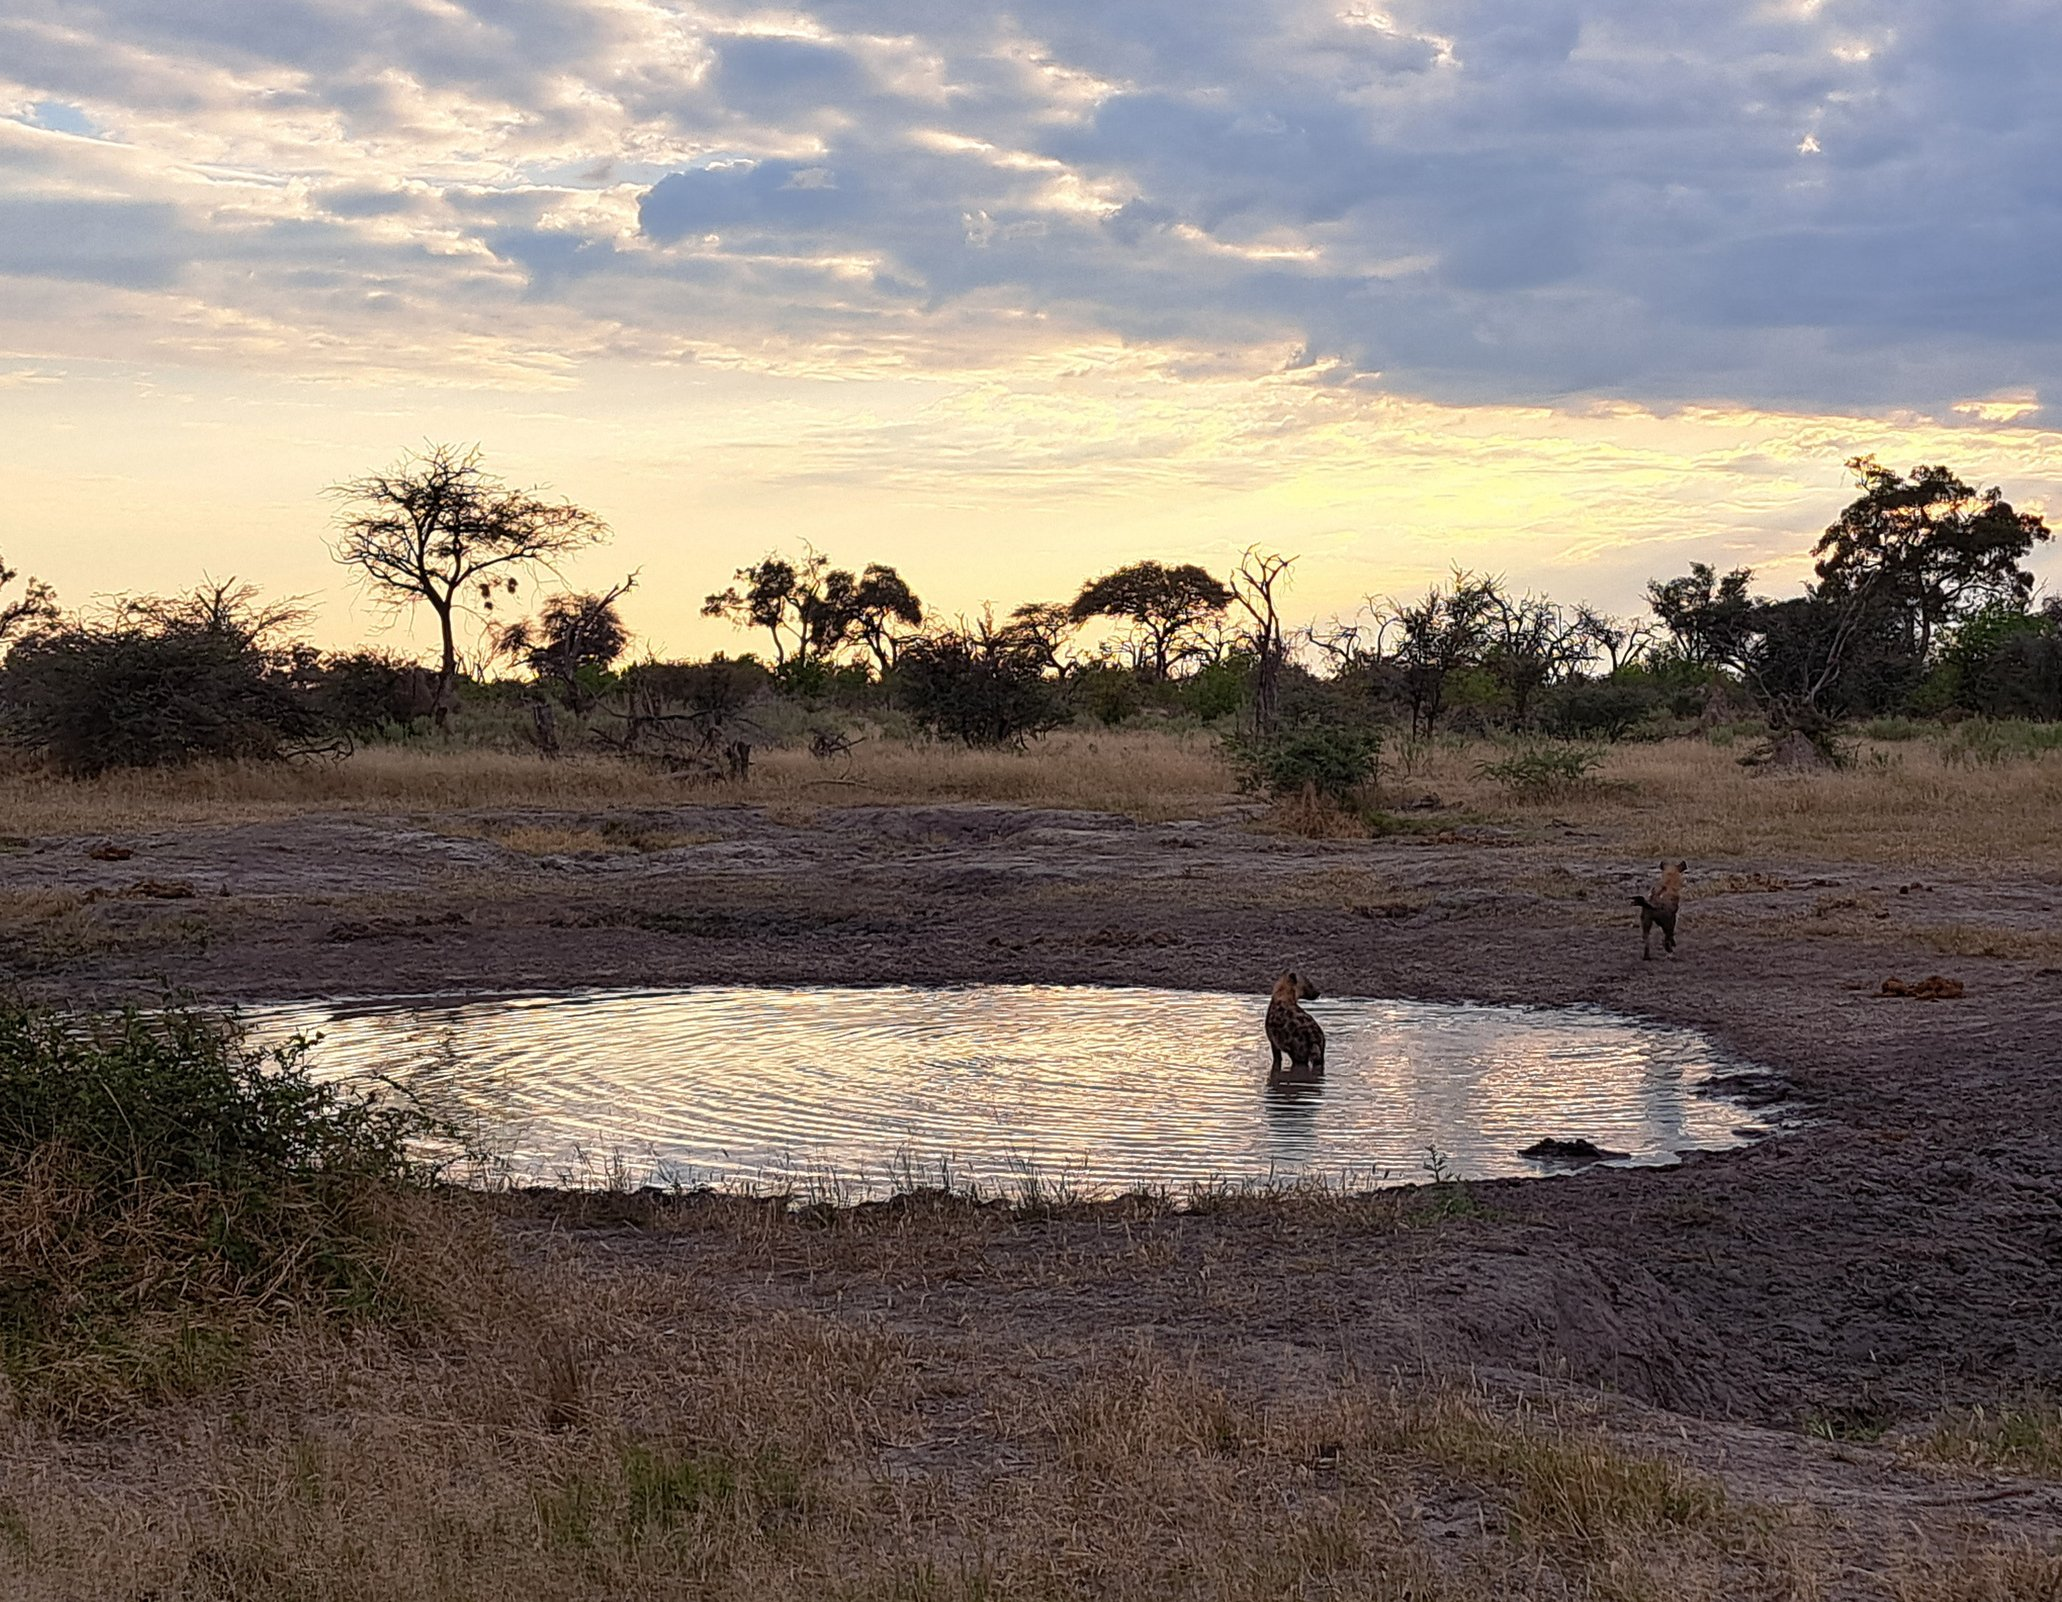
\includegraphics[width = \textwidth]{Figures/Pan}
  \caption{A pan as it can be found in Botswana right after the rainy season.
  This particular pan is comparably small at around 10 meters in diameter. Some
  of these pans dry out quickly, whereas others provide a source of water for
  the entire dry-season. Here, two spotted hyenas (\textit{Crocuta crocuta})
  take a quick bath.}
  \label{Pan}
 \end{center}
\end{figure}

\begin{table}[h]
  \begin{center}
  \caption{Overview of the spatial and temporal resolutions of the candidate satellite products.}
  \label{Satellite}
    \begin{threeparttable}[h]
      
\begin{tabular}[t]{llcc}
\toprule
Satellite & Availability & Spatial Resolution (m)\textsuperscript{*} & Temporal Resolution (days)\\
\midrule
Landsat 7 & 1999 – Present & 15 – 60 & 16\\
Landsat 8 & 2013 – Present & 15 – 100 & 16\\
Sentinel 2 & 2015 – Present & 10 – 60 & 5 – 10\textsuperscript{\dag}\\
\bottomrule
\end{tabular}

      \begin{tablenotes}
        \item \textsuperscript{*} \textit{Spatial resolutions of the same product can differ depending on the band.}
        \item \textsuperscript{\dag} \textit{Sentinel 2's revisitation duration decreased to 5 days after March 2017.}
      \end{tablenotes}
    \end{threeparttable}
  \end{center}
\end{table}

\noindent Our goal was to produce dynamically updated pan-maps that we could
overlay with GPS data of dispersing African wild dogs. Since most GPS data were
collected between 2015 and 2022, this implied that satellite data needed to be
available for the same period. At first glance, all satellite products appeared
to meet this criteria. However, Landsat 7's scan-line detector had been failing
since May 31, 2003, introducing data gaps between adjacent tiles, thus rendering
the product virtually unusable for our purposes (but see \citealp{Storey.2005}).
Sentinel 2 and Landsat 8, by contrast, appeared as viable alternatives, as both
of them spanned the desired period and did not exhibit any device failures.

\subsection{Evaluation of Landsat 8 and Sentinel 2}
\subsubsection{Training Polygons}

With Landsat 8 and Sentinel 2 imagery remaining, we conducted a preliminary
investigation to compare the two products and evaluate their suitability for our
needs. Specifically, we investigated how well we could remote sense pans using
either of the two products, utilizing supervised learning methods. For this, we
prepared a set of training polygons, consisting of the land cover classes
dryland, water, and wet-pans. Although our primary goal was to detect wet-pans,
we included the two other classes to facilitate the categorization of
reflectance values into distinct groups. Due to the large study area considered,
\textit{in situ} ground-truthing of the training polygons was impossible, and we
instead opted for \textit{on-screen selection} of training data. More
specifically, we utilized Google Earth to digitize areas that were clearly
identifiable as either dryland, water, or wet-pans. At the highest zoom level in
Google Earth, these categories are visually easy to tell apart
(\Cref{PanMapping}). To ensure a sharp distinction between wet-pans and dryland,
we traced several dryland polygons in areas that were seasonally covered by
water (\Cref{PanMapping}). Google Earth provides the date of any satellite map,
and so we could assign a timestamp to each training-polygon. This was necessary
to later match training polygons with Landsat or Sentinel data of the same date.
Google Earth's ability to display imagery from different dates furthermore
allowed us to generate a training dataset that comprised polygons that belonged
to different classes depending on the season. For example, a dryland polygon
obtained in the dry season could overlap with a wet-pan polygon obtained during
the rainy season. Overall, we generated \inputy{GeneralMetrics/TrainingTotal}
polygons of varying size and shape (\inputy{GeneralMetrics/TrainingDryland} on
dryland, \inputy{GeneralMetrics/TrainingWater} in water, and
\inputy{GeneralMetrics/TrainingWetpan} in wet-pans) for
\inputy{GeneralMetrics/TrainingDates} distinct dates (August 18, 2018, March 25,
2019, and July 24, 2021).

\begin{figure}[htpb]
 \begin{center}
  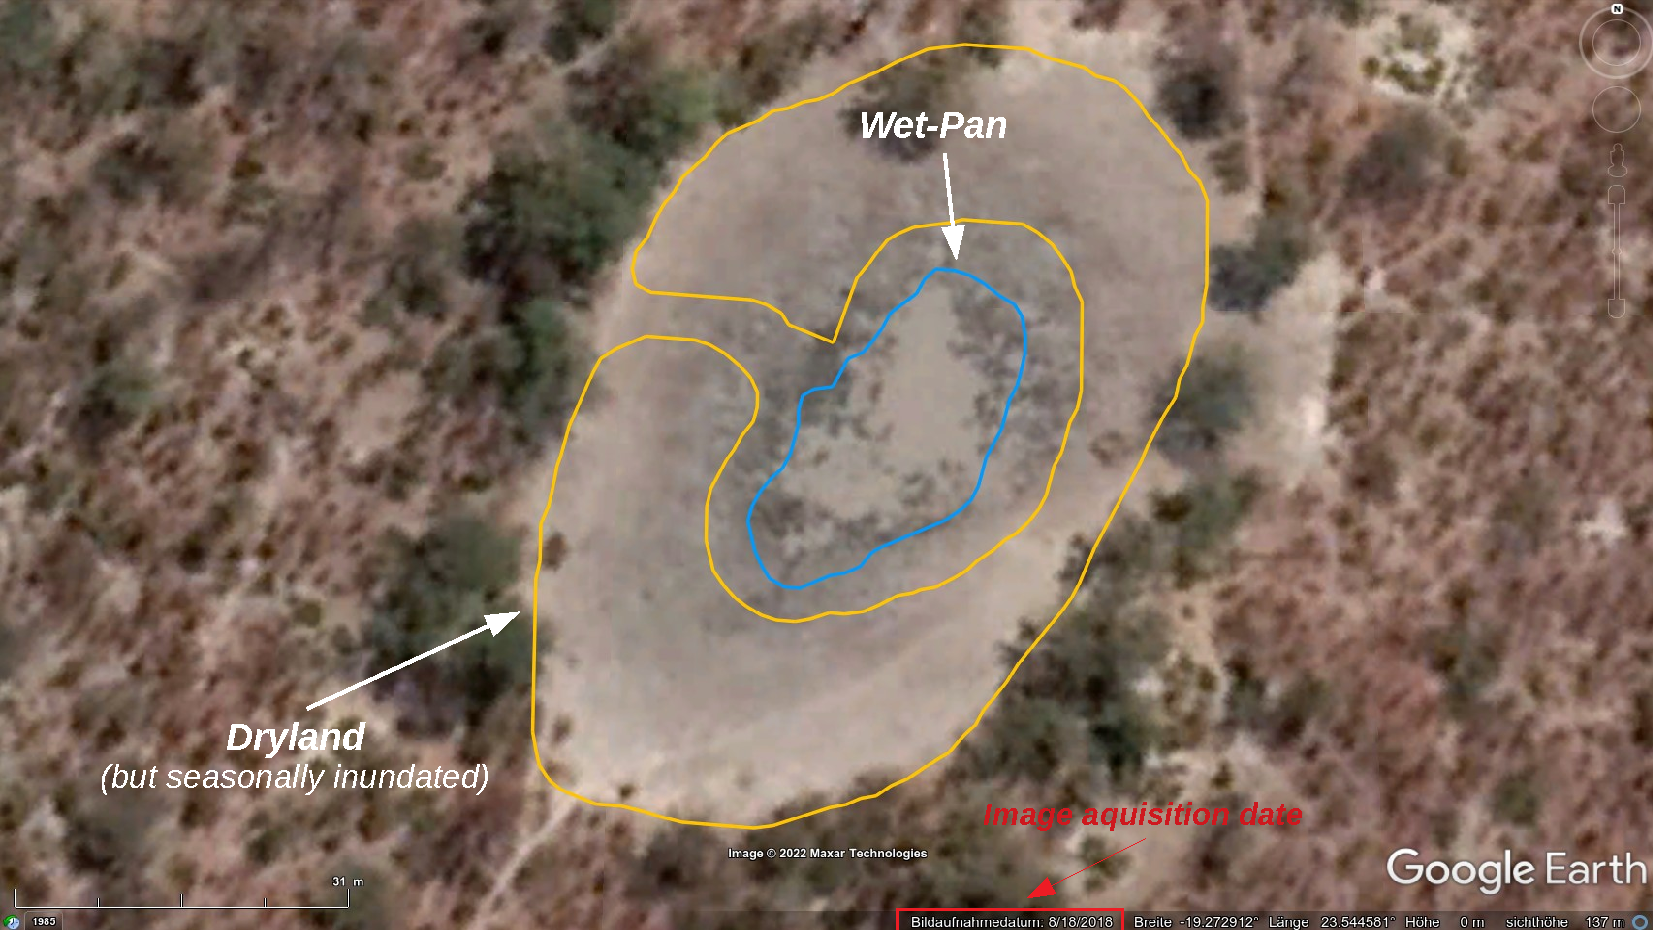
\includegraphics[width = \textwidth]{Figures/PanMapping.pdf}
  \caption{Example of a \textit{wet pan} and \textit{dryland} training polygon
  digitized on Google Earth. The extent of water can easily be gauged at the
  maximum zoom level in Google Earth. While the dryland polygon in this case
  covered an area that is seasonally covered by water, we placed other dryland
  polygons in areas that were never inundated. However, to ensure reliable
  differentiation between wet and dry pans, we included several dryland polygons
  located in dry pans.}
  \label{PanMapping}
 \end{center}
\end{figure}

\subsubsection{Satellite Data Download}
\label{Download}

We downloaded Landsat 8 imagery through Google Earth Engine using the
\texttt{rgee} \texttt{R}-package \citep{Aybar.2024} and used the associated
quality band to mask pixels classified as clouds or shadows. We also computed
several normalized difference indices (NDs), as listed in \Cref{ND}. To download
Sentinel 2 data, we used the \texttt{sen2r} \texttt{R}-package
\citep{Ranghetti.2020} which provides a standardized interface to download and
process Sentinel 2 imagery from the European Space Agency's data hub. Sentinel 2
data are available as either top-of-the-atmosphere (TOA, level 1C) or
bottom-of-the-atmosphere (BOA, level 2A) reflectance values. In analyses where
temporal trends are considered, the use of BOA reflectances is recommended, as
differences in reflectance properties due to atmospheric conditions are
accounted for \citep{Gilabert.1994, Vermote.2008, Chraibi.2022}. However, a
large portion of the publicly available Sentinel 2 data has not yet been
processed from level 1C to level 2A, requiring researchers to apply the
corrections themselves. Fortunately, the European Space Agency provides the
correction tool \texttt{sen2cor} for free \citep{Main-Knorn.2017}, which has
been integrated into the \texttt{R}-package \texttt{sen2r}
\citep{Ranghetti.2020}. We therefore applied the necessary corrections after
download for any product that hadn't already been corrected. Furthermore, we
used Sentinel 2's scene classification, to remove pixels classified as either
clouds or shadows. Finally, we computed the same ND-indices as for Landsat 8
(\Cref{ND}).

\begin{table}[h]
  \begin{center}
  \caption{We computed normalized difference indices between certain bands,
  hoping they would improve the land-cover classifiers. Depending on the
  satellite, we used different bands to compute similar indices. The function to
  compute a normalized difference between bands $b_1$ and $b_2$ is given by
  $\frac{b1 - b2}{b1 + b2}$.}
  \label{ND}
  \begin{threeparttable}[h]
    
\begin{tabular}[t]{lcc}
\toprule
\multicolumn{1}{c}{} & \multicolumn{2}{c}{Bands} \\
\cmidrule(l{3pt}r{3pt}){2-3}
Index & Landsat 8 & Sentinel 2\\
\midrule
NDWI & B3, B5 & B3, B8\\
NDMI & B5, B6 & B8, B11\\
NDSI & B3, B6 & B3, B11\\
BEST & B3, B7 & B3, B12\\
\bottomrule
\end{tabular}

  \end{threeparttable}
  \end{center}
\end{table}

\subsubsection{Land Cover Classifiers}

To train a land-cover classifier, we generated 3,000 random points within
training polygons following a stratified equal random sampling scheme
\citep{Shetty.2021}. That is, we ensured that 1,000 random points were sampled
per training category. Stratified random sampling was necessary to ensure that
wet-pans, our category of interest, was sampled frequently enough, as it
represented a minority class, only making up of
(\inputy{GeneralMetrics/PercentageTrainingWetpan}\%) the total training area.
Stratified equal random sampling has been shown to provide good class-level
accuracy for minority classes \citep{Shetty.2021}, so we deemed this approach
suitable for our purposes. We also kept track of the dates of the underlying
polygons from which random points were generated. At each random point, we then
extracted reflectance values of Sentinel 2 and Landsat 8 data that temporally
aligned with the date assigned to the random point (\Cref{Reflectances}a). For
instance, if a random point fell into a polygon that was digitized using a
Google Earth image generated on Aug 18, 2018, we extracted values from the
Sentinel 2 and Landsat 8 layers that were closest to that date. Finally, we
parameterized a Random Forest (RF) classifier using the \texttt{R}-package
\texttt{randomForest} \citep{Cutler.2024} and a Classification and Regression
Tree (CART) classifier using the \texttt{R}-package \texttt{rpart}
\citep{Therneau.2024b}. In both cases, we included all bands, as well as derived
ND-indices (\Cref{ND}) as explanatory covariates. We visualized the decision
trees for the CART classifiers (\Cref{Reflectances}b) and variable importance
for the RF models (\Cref{Reflectances}c) to investigate the importance of
different bands or indices in separating the three classes. To compute variable
importance we used the \texttt{R}-package \texttt{caret} \citep{Kuhn.2008}.

\begin{figure}[htpb]
 \begin{center}
  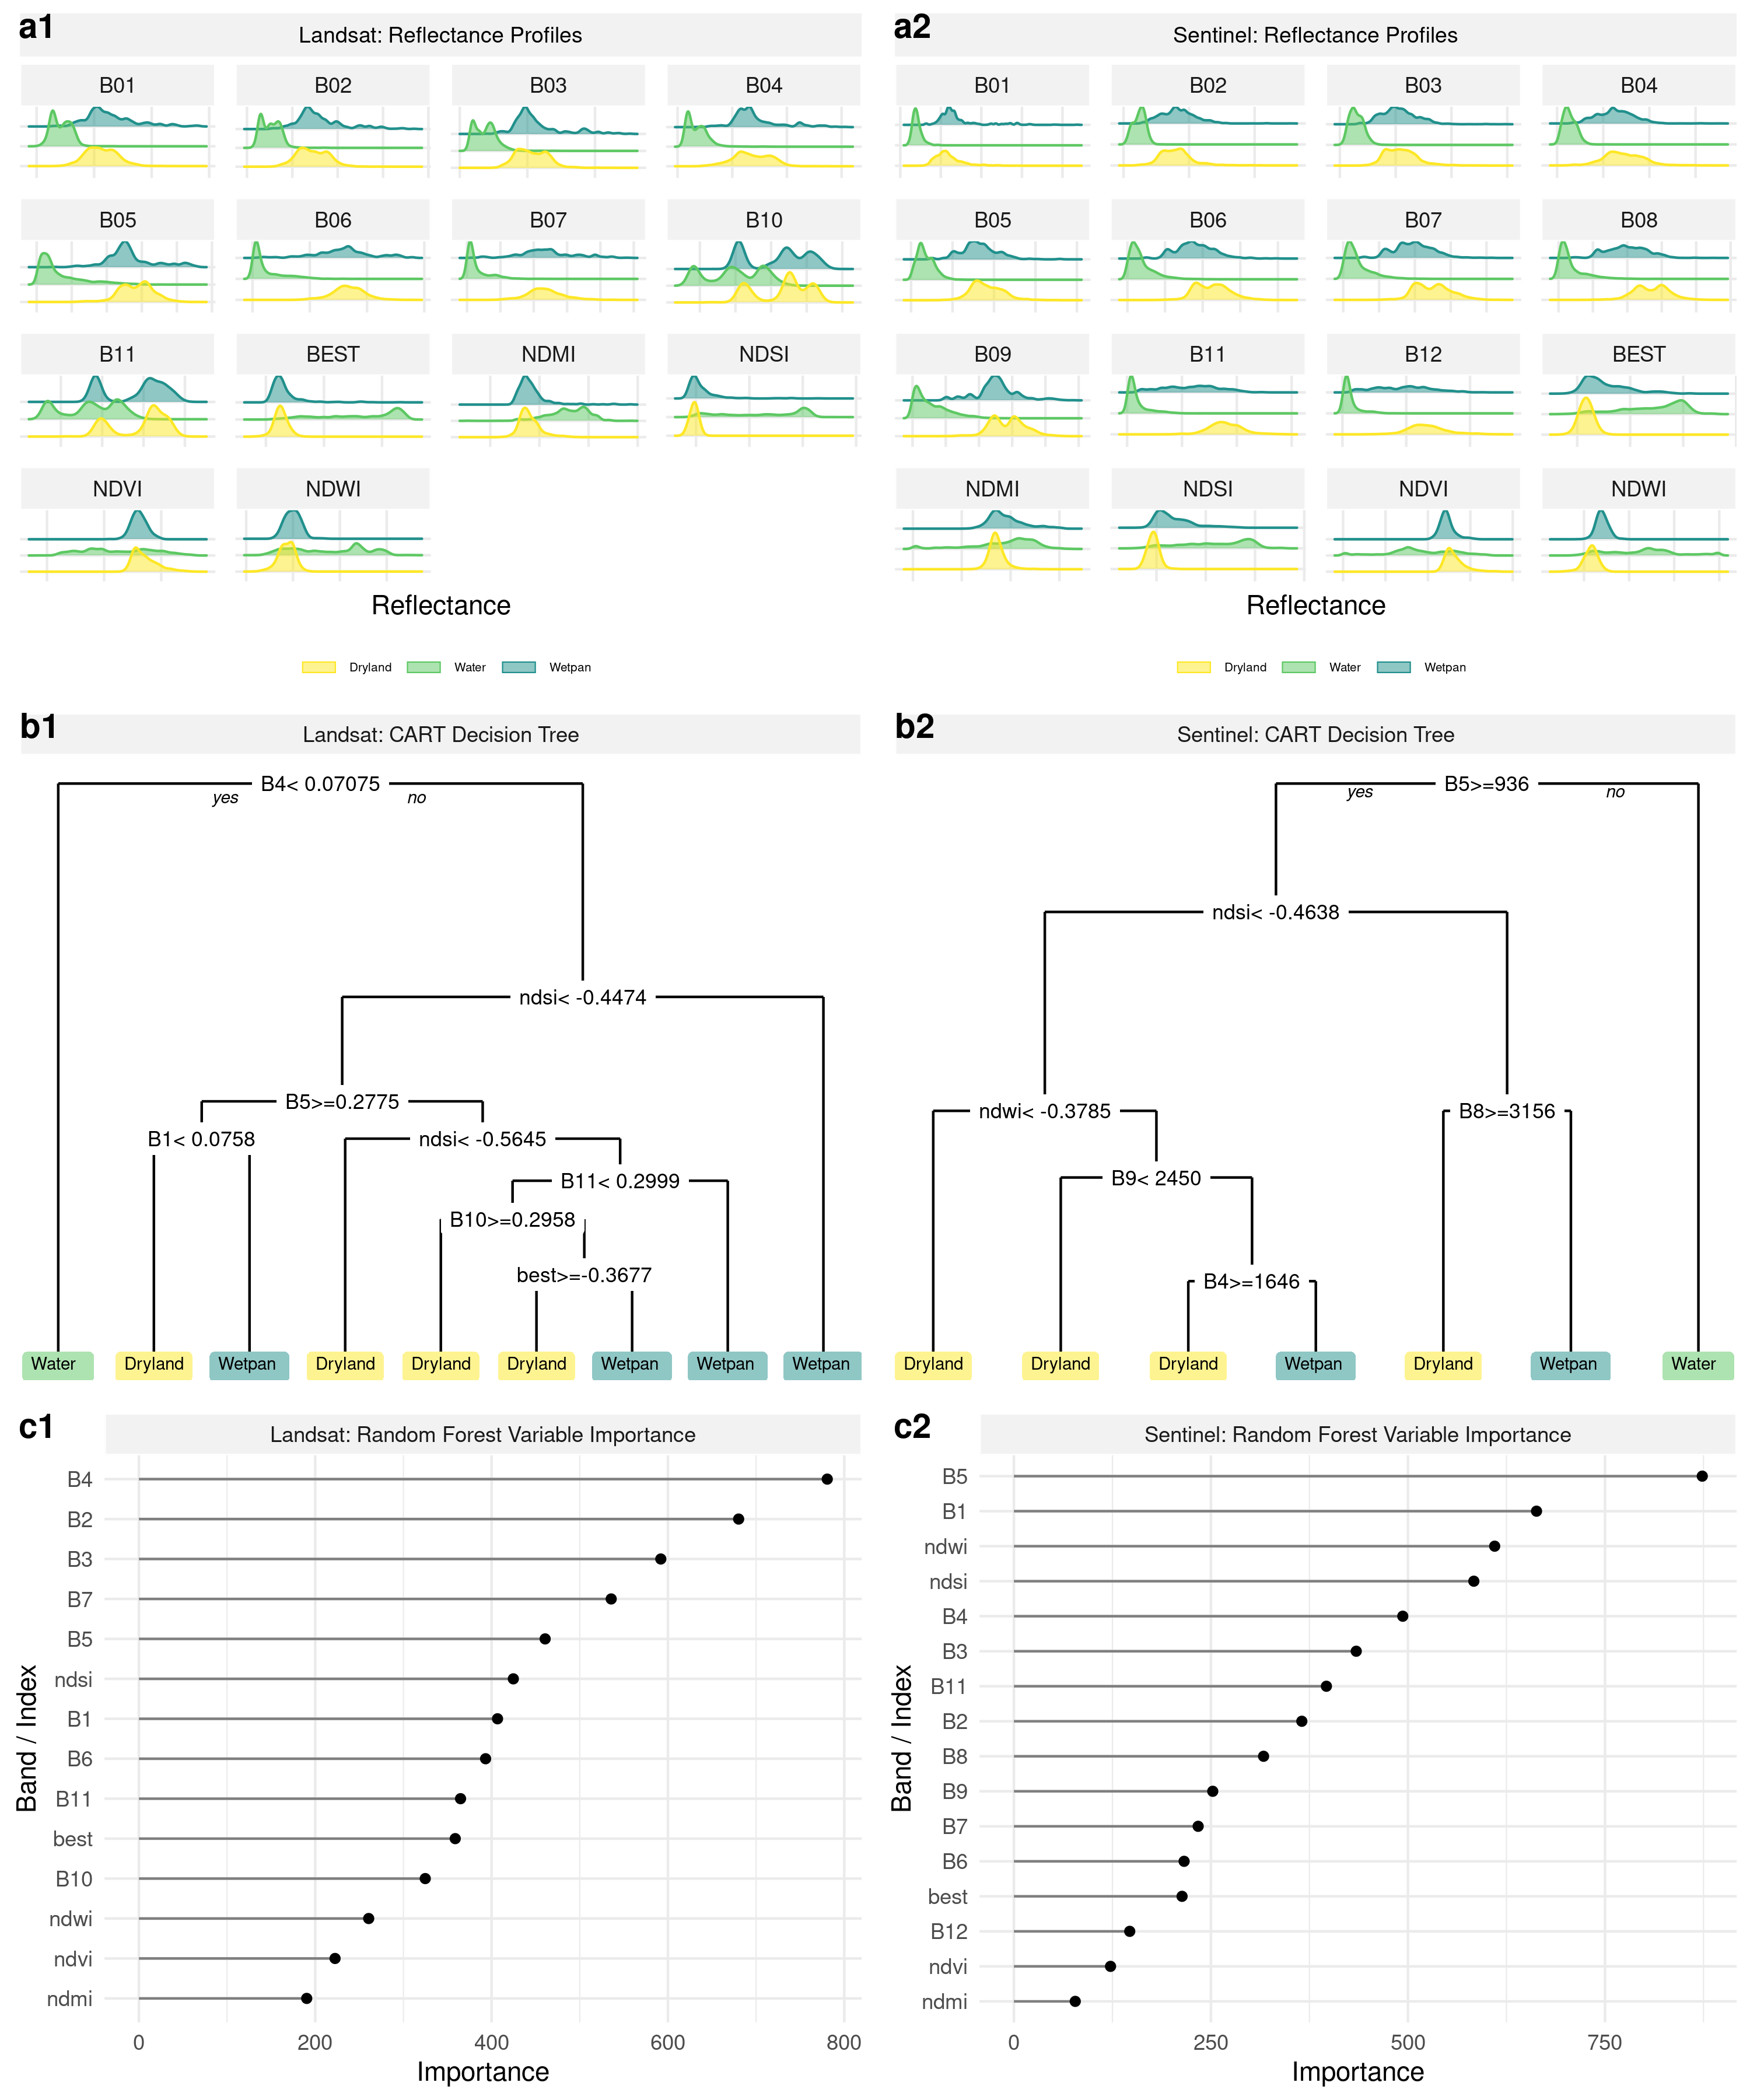
\includegraphics[width = \textwidth]{Figures/Reflectances.png}
  \caption{Reflectance properties of the Landsat 8 (a1) and Sentinel 2 (a2)
  bands and NDs at the extracted training points for each of the three
  categories (colored). Based on extracted reflectance values we parametrized
  Classification and Regression Tree models (b1 and b2) as well as Random Forest
  models (c1 and c2).}
  \label{Reflectances}
 \end{center}
\end{figure}

\subsubsection{Validation and Comparison}

To validate the predictive power of the two classifiers across the two datasets,
we employed 5-fold cross-validation. For this, we randomly split the data into 5
groups and repeatedly fitted both classification models using 80\% of the data,
to then predict land cover categories in the remaining 20\%. We generated
confusion matrices to contrast true and predicted labels and computed estimates
of the classifier's specificity, sensitivity, and overall accuracy. The results
from this validation show that both classifiers achieve $\geq$ 90\% accuracy
across both satellite products (\Cref{ClassificationValidation}). In fact, the
RF classifier resulted in an overall accuracy of 99\% on Sentinel 2 data.

\begin{figure}[htpb]
 \begin{center}
  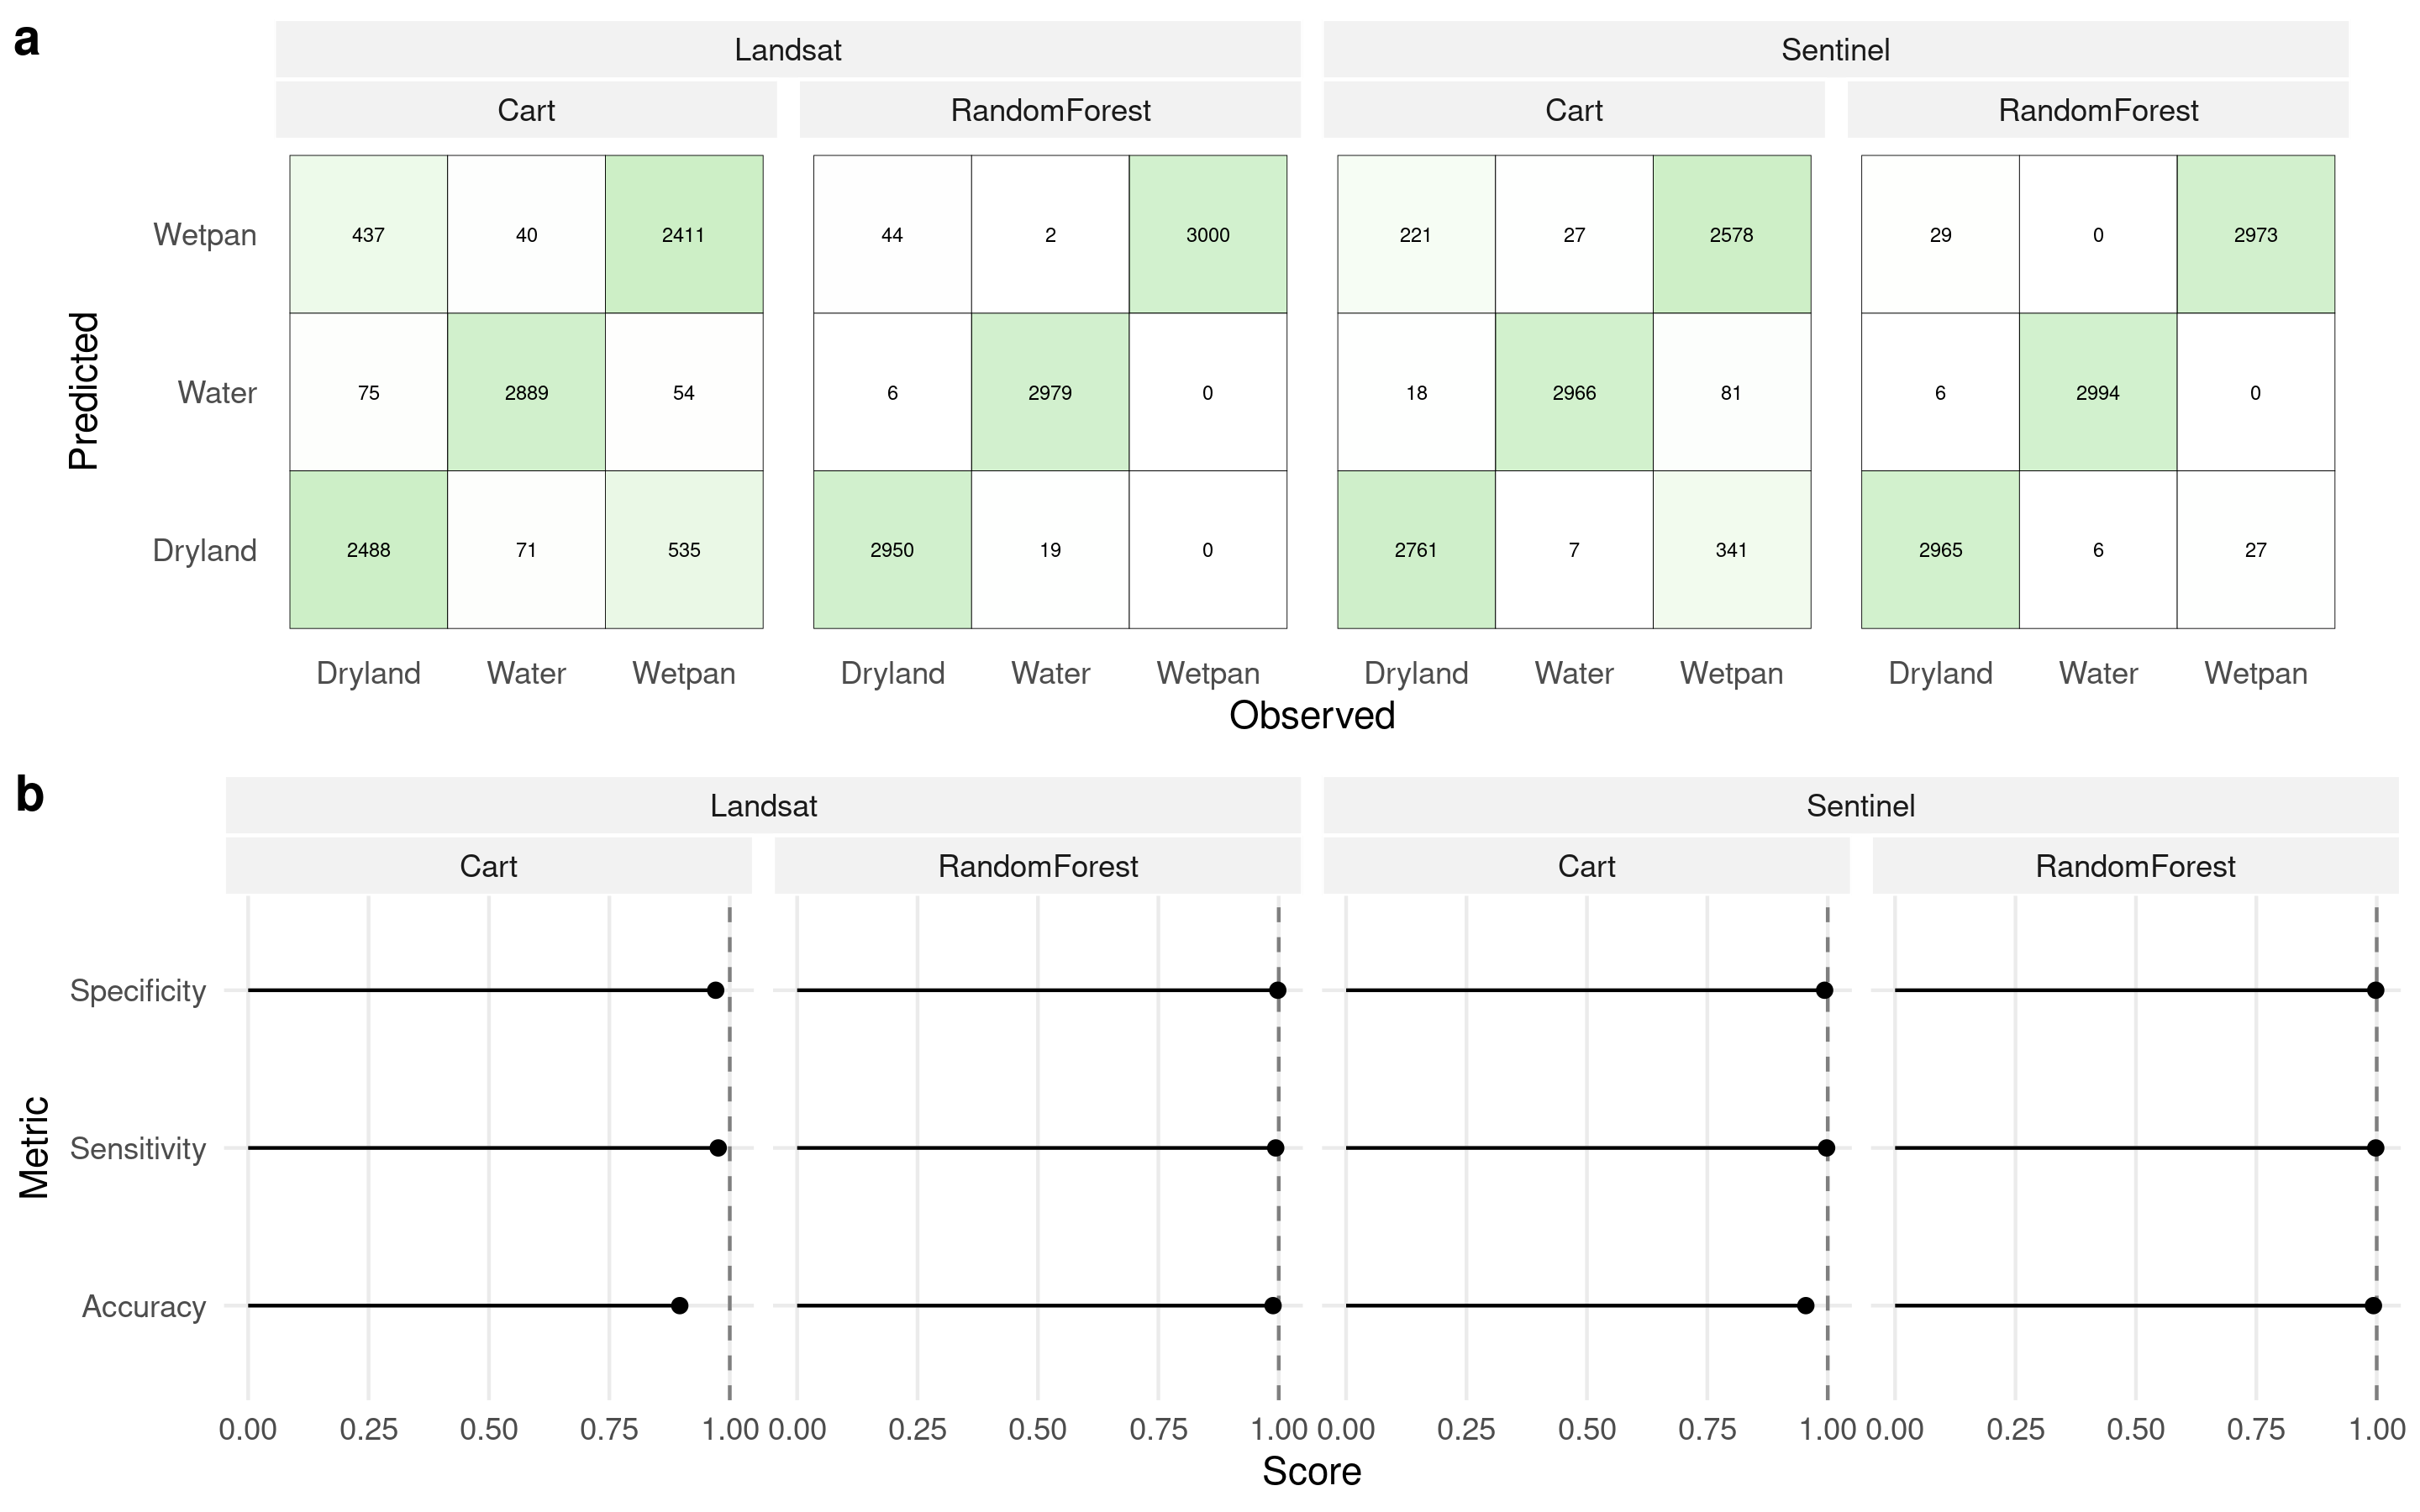
\includegraphics[width = \textwidth]{Figures/ClassificationValidation.png}
  \caption{Confusion matrices (a) and derived performance metrics (b) for the
  CART and RF classifiers for both the Landsat 8 and Sentinel 2 datasets.}
  \label{ClassificationValidation}
 \end{center}
\end{figure}

\subsection{Bulk Download}

Although both Landsat 8 and Sentinel 2 provided very good results, we considered
Sentinel 2 data to be marginally superior, mainly due to Sentinel's higher
temporal and spatial resolution. A higher temporal resolution was key to
compensate missing data from satellite mages obtained on cloudy days and
therefore pivotal in achieving cloud free monthly composites. We therefore
decided to download Sentinel 2 data for the period during which we also
collected GPS data of dispersing individuals. Instead of downloading all
Sentinel 2 tiles overlapping with our study area and matching the study-period,
we created a spatio-temporal moving window (\Cref{MovingWindows}). This window
was updated each month and comprised all GPS locations collected during that
month, buffered by a 100 km radius. We then identified Sentinel 2 tiles
intersecting with each of the monthly updated moving windows
(\Cref{MovingWindows2}). This resulted in a list of
\inputy{GeneralMetrics/NumberTilesTotal} tiles that needed to be downloaded,
\inputy{GeneralMetrics/NumberTiles2A} of which were already corrected to BOA
reflectances, while the remaining \inputy{GeneralMetrics/NumberTiles1C} tiles
still needed to be corrected. The download followed the same procedure and
included the same corrections (from TOA to BOA, and cloud masking) as outlined
in \Cref{Download} using the \texttt{sen2r} package in \texttt{R}
\citep{Ranghetti.2020}. Upon completion of the download and pre-processing, we
applied the trained RF classifer to obtain binary ``pan-maps'', showing the
spatial distribution of ephemeral water bodies. To generate monthly composites,
we merged all pan-maps falling into the same month and retained pans if they
were detected in at least 50\% of the overlapping tiles. Finally, we generated
``distance-to-pan'' maps using the \texttt{distance} function from the
\texttt{terra} package in \texttt{R} \citep{Hijmans.2024}.

\begin{figure}[htpb]
 \begin{center}
  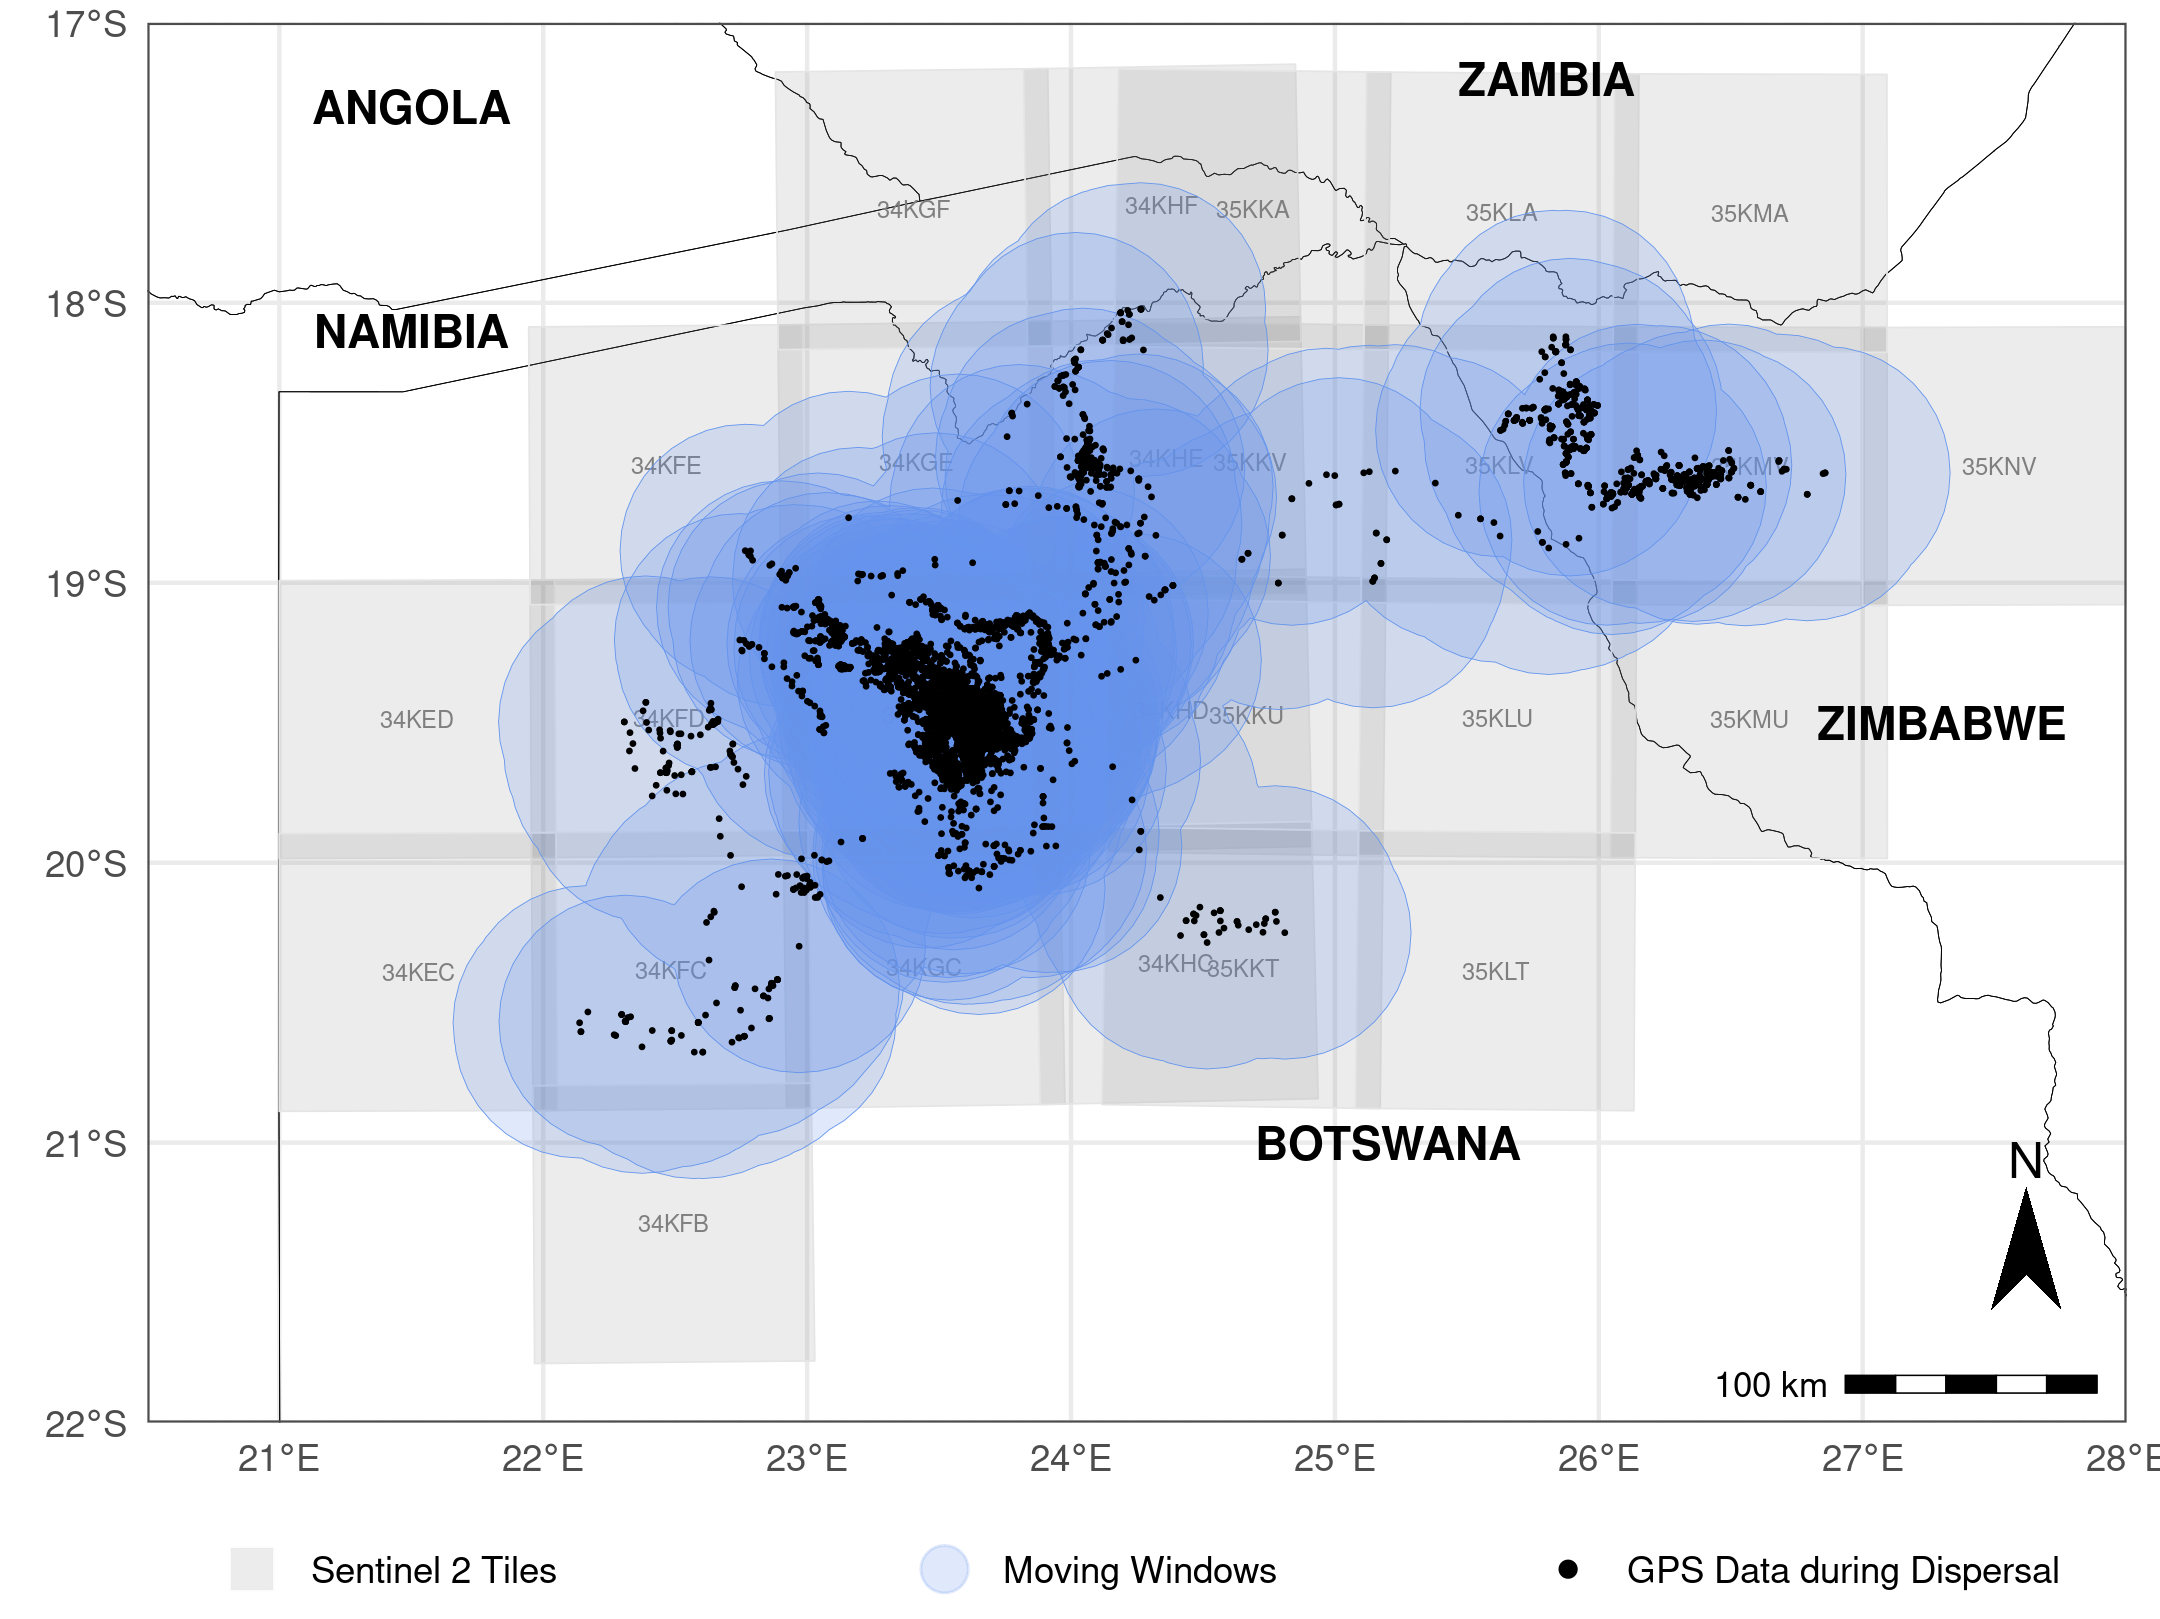
\includegraphics[width = \textwidth]{Figures/MovingWindows.png}
  \caption{To reduce the number of Sentinel 2 tiles that we needed to download,
  we generated a monthly updated spatio-temporal moving window that comprised
  all GPS data of dispersing wild dogs (black dots) during the respective month,
  buffered by a 100 km radius. Based on the so created moving windows (in blue),
  we identified all overlapping Sentinel 2 tiles (tiles in gray) that we needed
  to download each month, which resulted in a total of 2,226 tiles.}
  \label{MovingWindows}
 \end{center}
\end{figure}

\begin{figure}[htpb]
 \begin{center}
  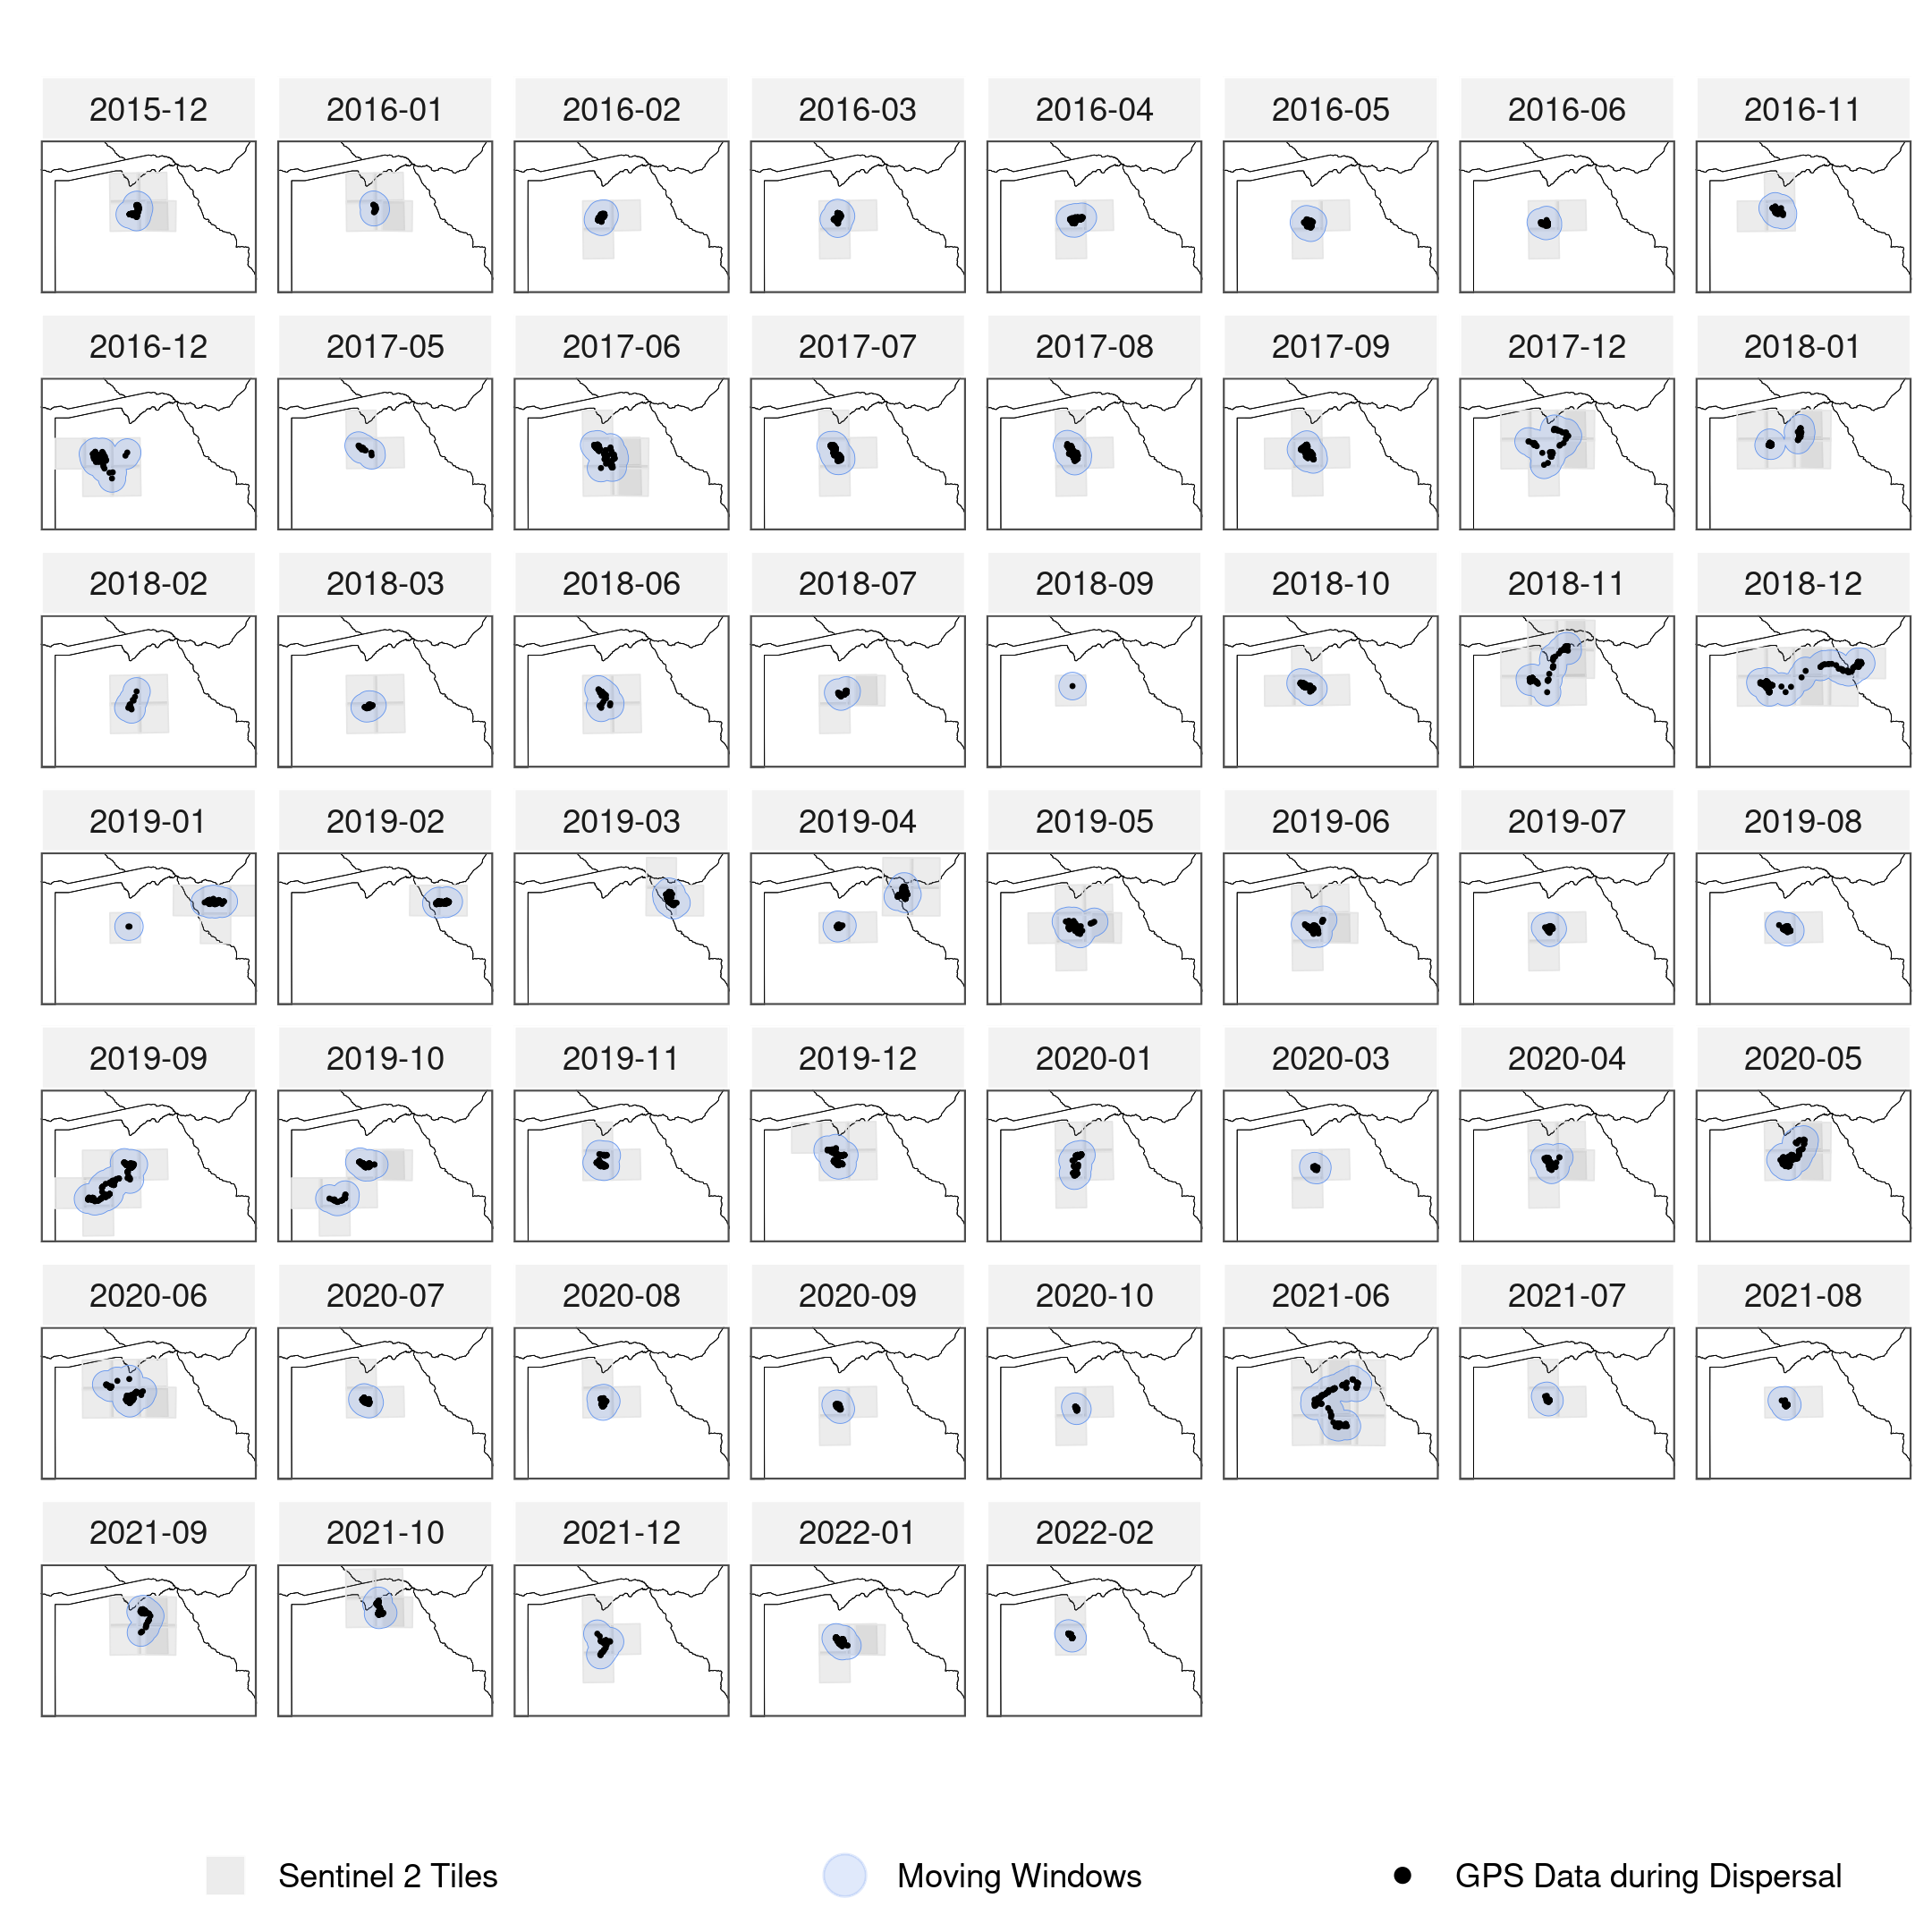
\includegraphics[width = \textwidth]{Figures/MovingWindows2.png}
  \caption{This figure shows the moving windows generated for each month, as
  well as the underlying GPS data and overlapping Sentinel 2 tiles that we
  ultimately downloaded and combined into monthly composites.}
  \label{MovingWindows2}
 \end{center}
\end{figure}

%------------------------------------------------------------------------------
%	Appendix S2: Moonlight
%------------------------------------------------------------------------------
\newpage
\section{Moon Illumination}

We used the \texttt{R}-package \texttt{moonlit} \citep{Smielak.2023} to obtain
estimates of moon illumination at 5 minute intervals at the average location of
dispersal GPS data (lon = of 23.5, lat = -19.0; \Cref{Moonlight}). The
\texttt{moonlit} package is currently not on \texttt{CRAN}, but can be installed
from GitHub (\url{https://github.com/msmielak/moonlit}). Besides providing
information on the moon cycle, this package also allows estimating the amount of
moonlight illumination on the ground. For instance, even during full-moon
nights, the moon may only appear at a low angle in the sky, thus providing
minimal illumination. Estimates from the \texttt{moonlit} package can therefore
be viewed as biologically more relevant. To match the temporal resolution of our
GPS data during dispersal, we calculated four hourly moonlight summaries.
Specifically, we computed if an interval fell into nighttime and the average
amount of moon-illumination during the four hours.

\begin{figure}[htpb]
 \begin{center}
  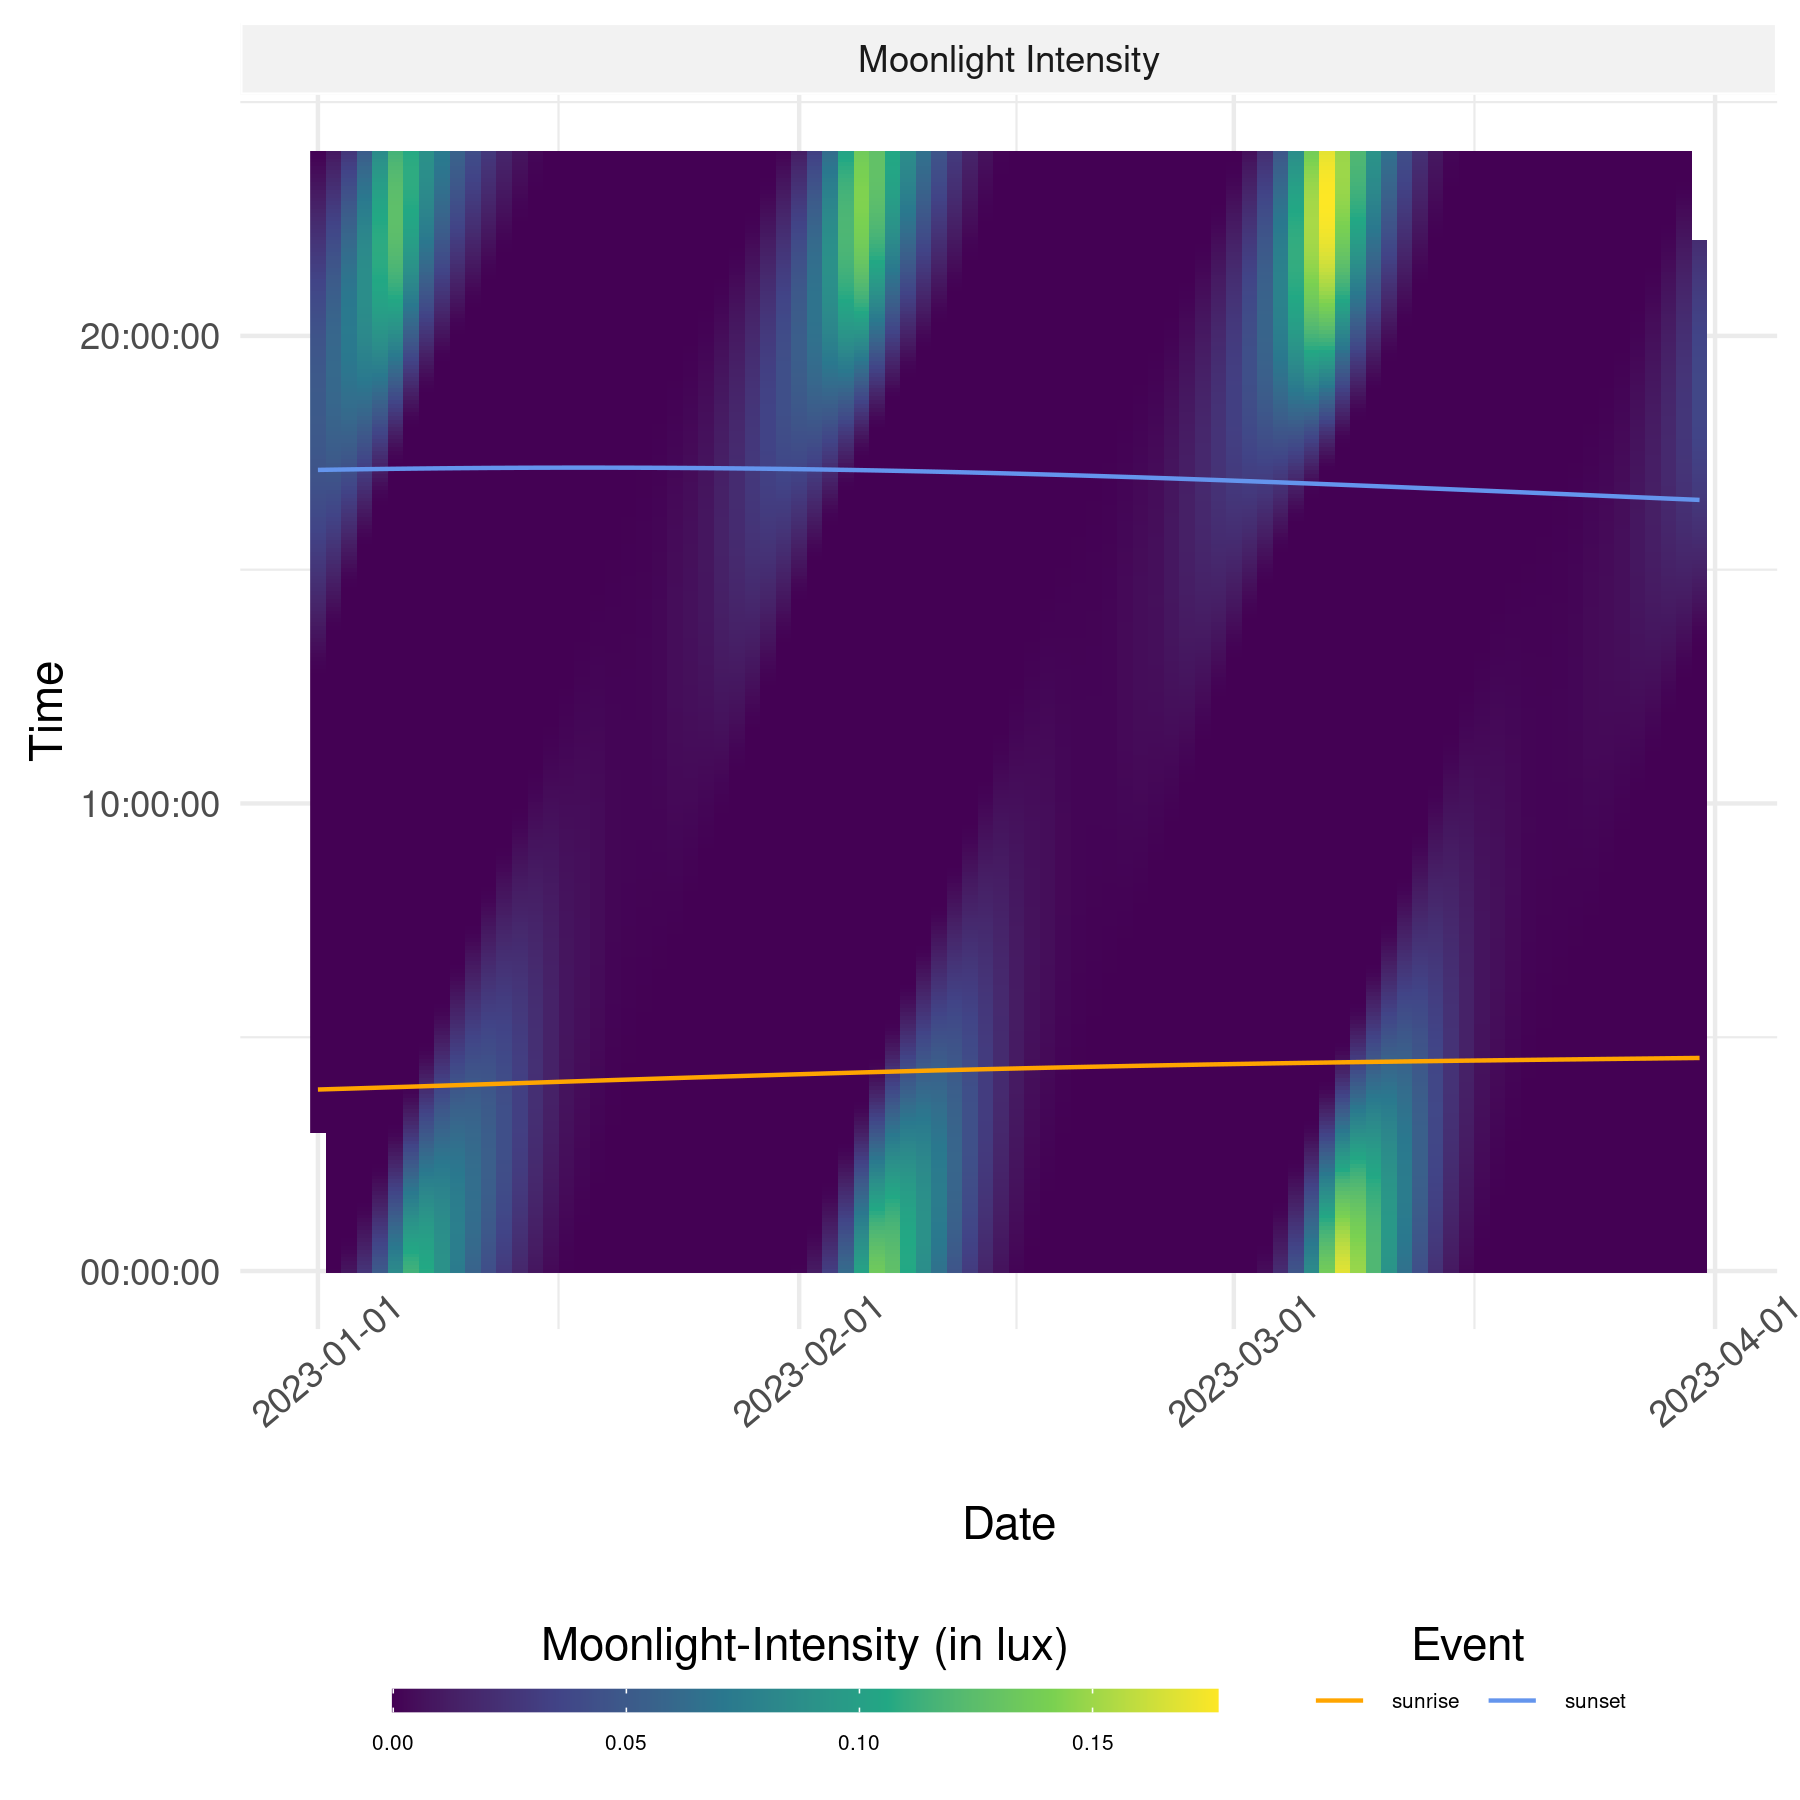
\includegraphics[width = 0.75\textwidth]{Figures/Moonlight.png}
  \caption{Moonlight intensity as estimated from the \texttt{moonlit} package
  \citep{Smielak.2023} in \texttt{R}, calculated for several example timestamps
  in 2023.}
  \label{Moonlight}
 \end{center}
\end{figure}

%------------------------------------------------------------------------------
%	Appendix S3: Light-Type of Each Step
%------------------------------------------------------------------------------
\newpage
\section{Light-Type}

\begin{figure}[htpb]
 \begin{center}
  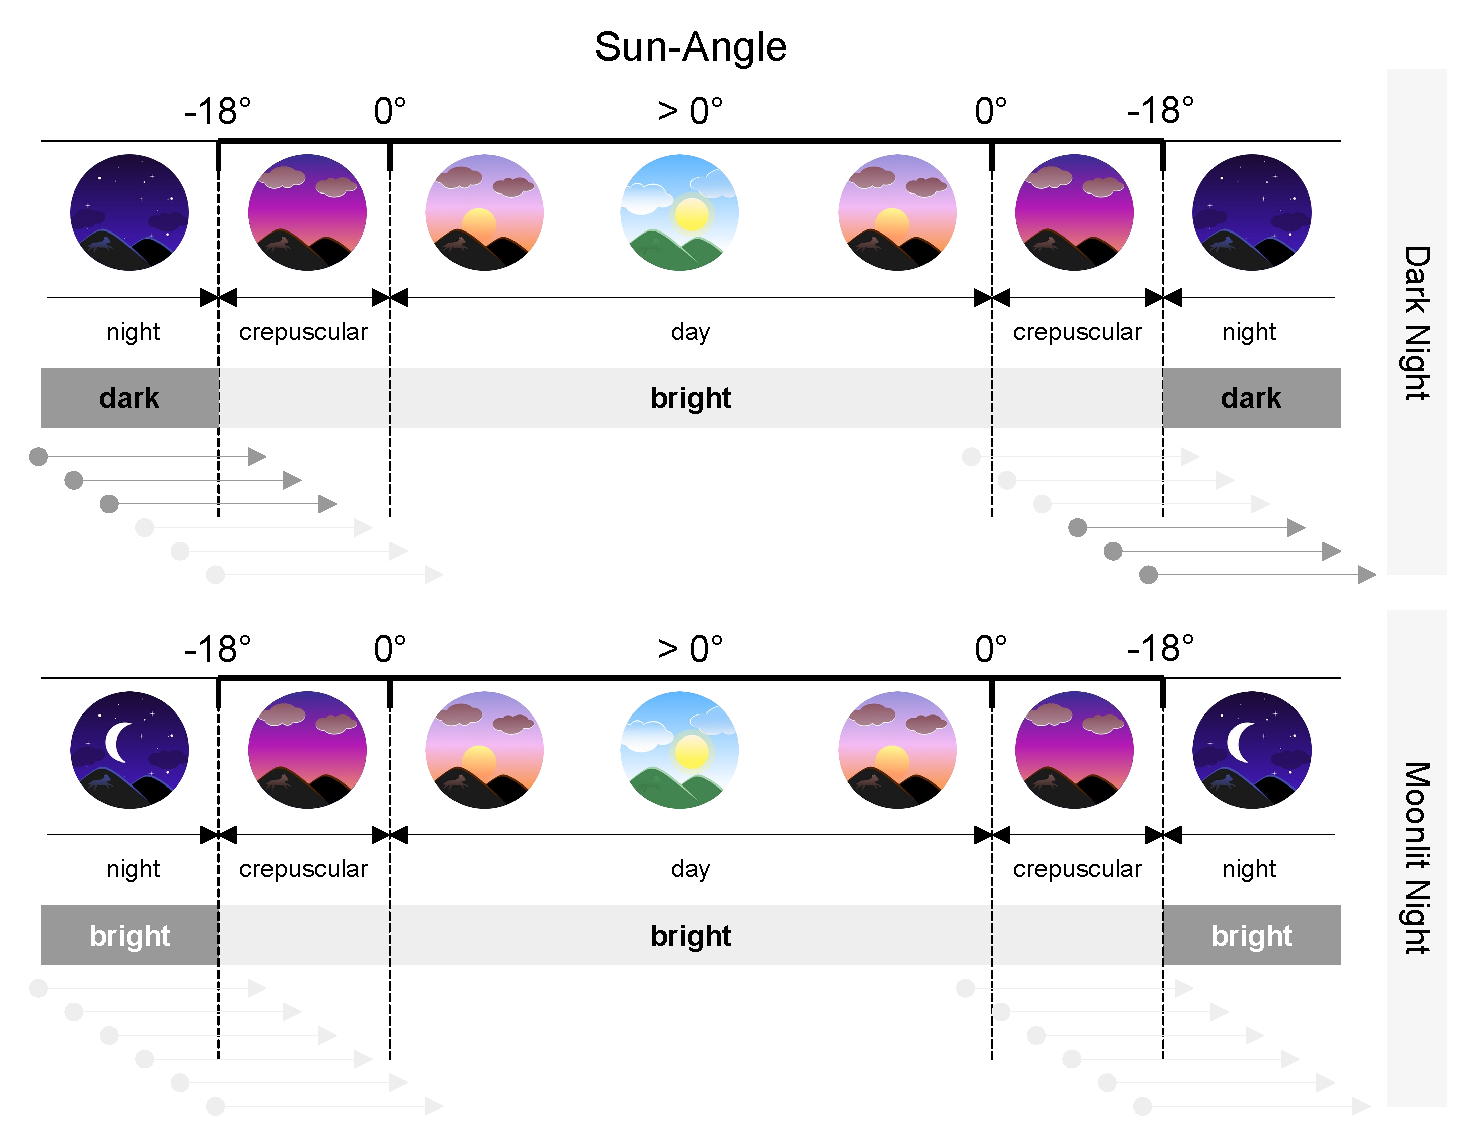
\includegraphics[width = \textwidth]{Figures/Light.pdf}
  \caption{Schematic illustration of how we categorized steps into \textit{dark}
  and \textit{bright} steps. First, we used the \texttt{suncalc} and
  \texttt{moonlit} packages to obtain estimates of the sun-angle and moon
  illumination at 5 minute intervals for each date of interest. Whenever the sun
  angle was $\leq $ -18\degree, we deemed the respective period to be at night.
  A night was either bright (moon illumination $>$ 0.02 of maximum illumination)
  or dark (moon illumination $\leq$ 0.02 of maximum illumination). Any other
  period was considered to provide enough illumination for wild dogs to move and
  therefore considered as bright. Since each step covered a time-span of
  approximately four hours, we defined a step as bright if at least 25\% (i.e.,
  one hour) of it occurred during a bright period. The gray arrows represent
  some example steps that are categorized as bright (light gray) or dark (dark
  gray).}
  \label{Light}
 \end{center}
\end{figure}

%------------------------------------------------------------------------------
%	Appendix S4: Movement Model Results
%------------------------------------------------------------------------------
\newpage
\section{Movement Model Results}

\begin{table}[htpb]
 \begin{center}
  \caption{Estimates obtained using the \textbf{simple model formula} (no
  interactions) and \textbf{static} covariates. GPS Data were either pooled
  across seasons (labeled ``all'') or split into wet and dry season. Only
  underlined covariates differed between the static and dynamic configurations.}
  \label{ModelsStaticSimple}
   \begin{threeparttable}
   \inputy{Figures/MovementModelStaticSimple.tex}
   \end{threeparttable}
 \end{center}
\end{table}

\begin{table}[htpb]
 \begin{center}
  \caption{Estimates obtained using the \textbf{simple model formula} (no
  interactions) and \textbf{dynamic} covariates. GPS Data were either pooled
  across seasons (labeled ``all'') or split into wet and dry season. Only
  underlined covariates differed between the static and dynamic configurations.}
  \label{ModelsDynamicSimple}
   \begin{threeparttable}
   \inputy{Figures/MovementModelDynamicSimple.tex}
   \end{threeparttable}
 \end{center}
\end{table}

\begin{table}[htpb]
 \begin{center}
  \caption{Estimates obtained using the \textbf{complex model formula} (with
  interactions) and \textbf{static} covariates. GPS Data were either pooled
  across seasons (labeled ``all'') or split into wet and dry season. Only
  underlined covariates differed between the static and dynamic configurations.}
  \label{ModelsStaticFull}
   \begin{threeparttable}
   \inputy{Figures/MovementModelStaticFull.tex}
   \end{threeparttable}
 \end{center}
\end{table}

\begin{table}[htpb]
 \begin{center}
  \caption{Estimates obtained using the \textbf{complex model formula} (with
  interactions) and \textbf{dynamic} covariates. GPS Data were either pooled
  across seasons (labeled ``all'') or split into wet and dry season. Only
  underlined covariates differed between the static and dynamic configurations.}
  \label{ModelsDynamicFull}
   \begin{threeparttable}
   \inputy{Figures/MovementModelDynamicFull.tex}
   \end{threeparttable}
 \end{center}
\end{table}

%------------------------------------------------------------------------------
%	Appendix S5: Stability with Regards to Number of Random Steps
%------------------------------------------------------------------------------
\newpage
\section{Number of Random Steps}

\begin{figure}[htpb]
 \begin{center}
  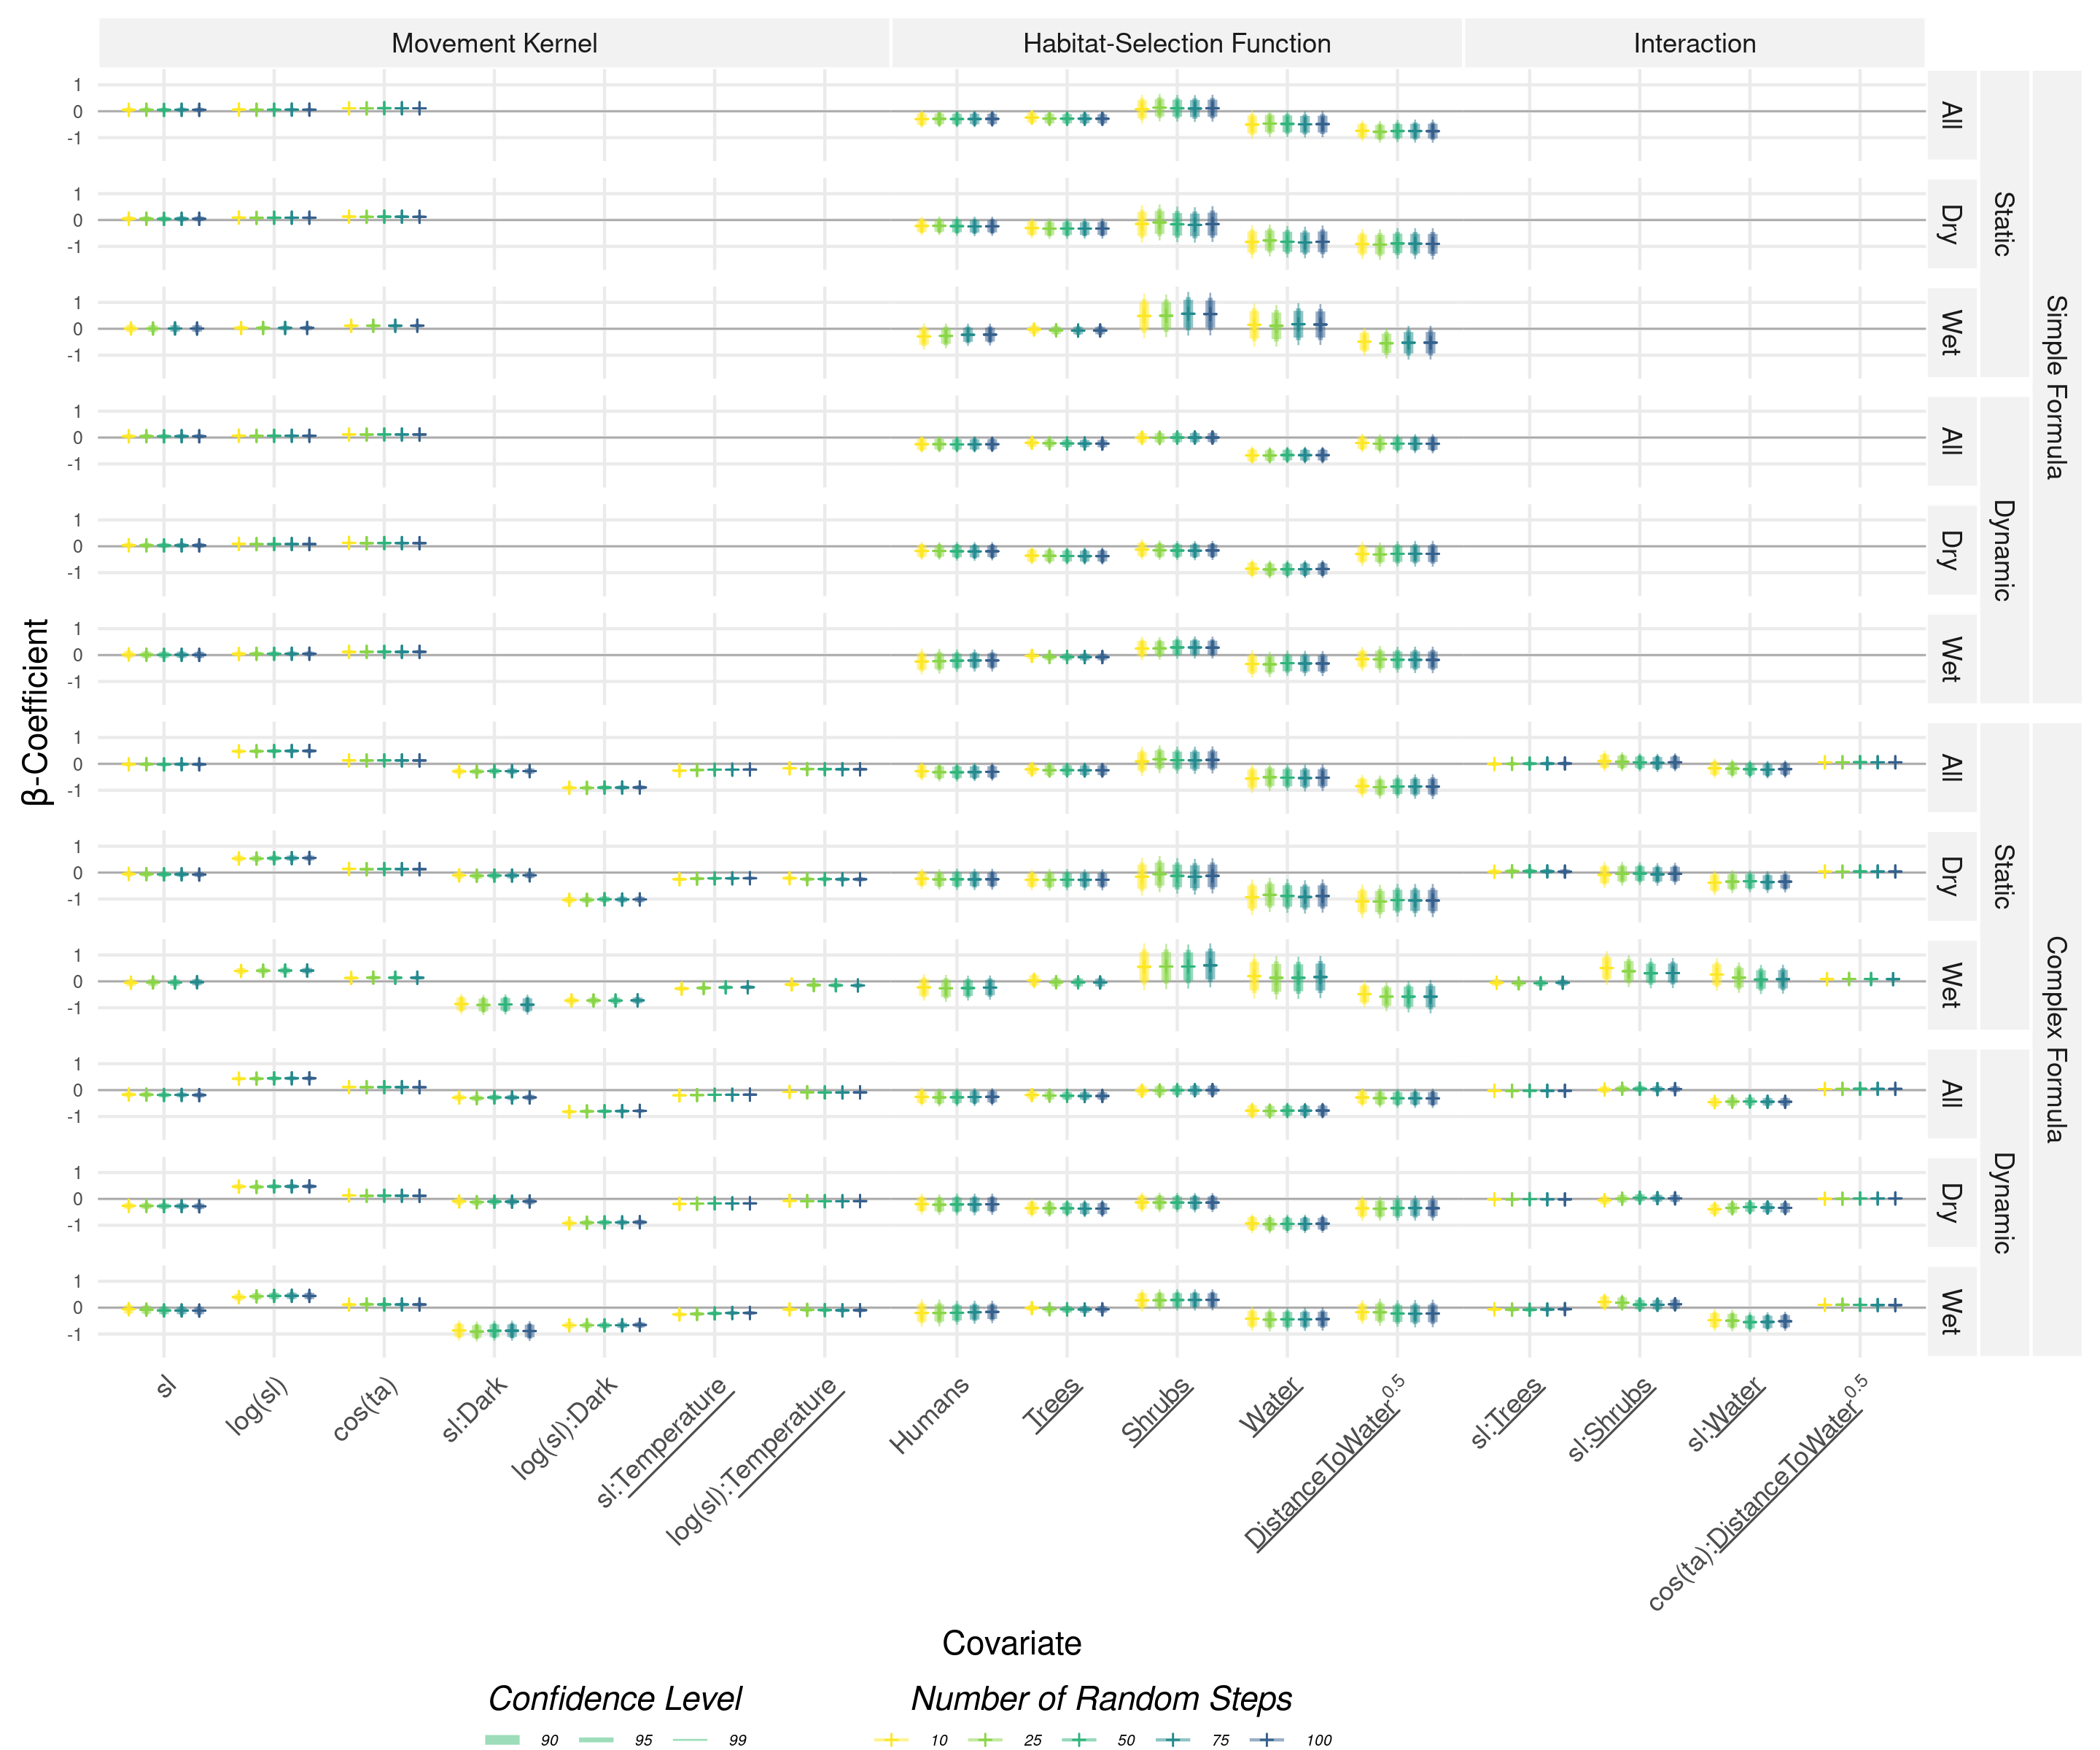
\includegraphics[width = \textwidth]{Figures/Stability.png}
  \caption{Results from the integrated step-selection models when considering
  different numbers of random steps. Results are shown for the simple and
  complex formulas for all configurations of fitting covariates (static vs dry)
  and model seasons (all vs. wet + dry). For some design combinations, models
  failed to converge and thus dropped from the figure.}
  \label{Stability}
 \end{center}
\end{figure}

%------------------------------------------------------------------------------
%	Appendix S6: Dispersal Model Interpretation
%------------------------------------------------------------------------------
\newpage
\section{Model Interpretation}

\begin{figure}[htpb]
 \begin{center}
  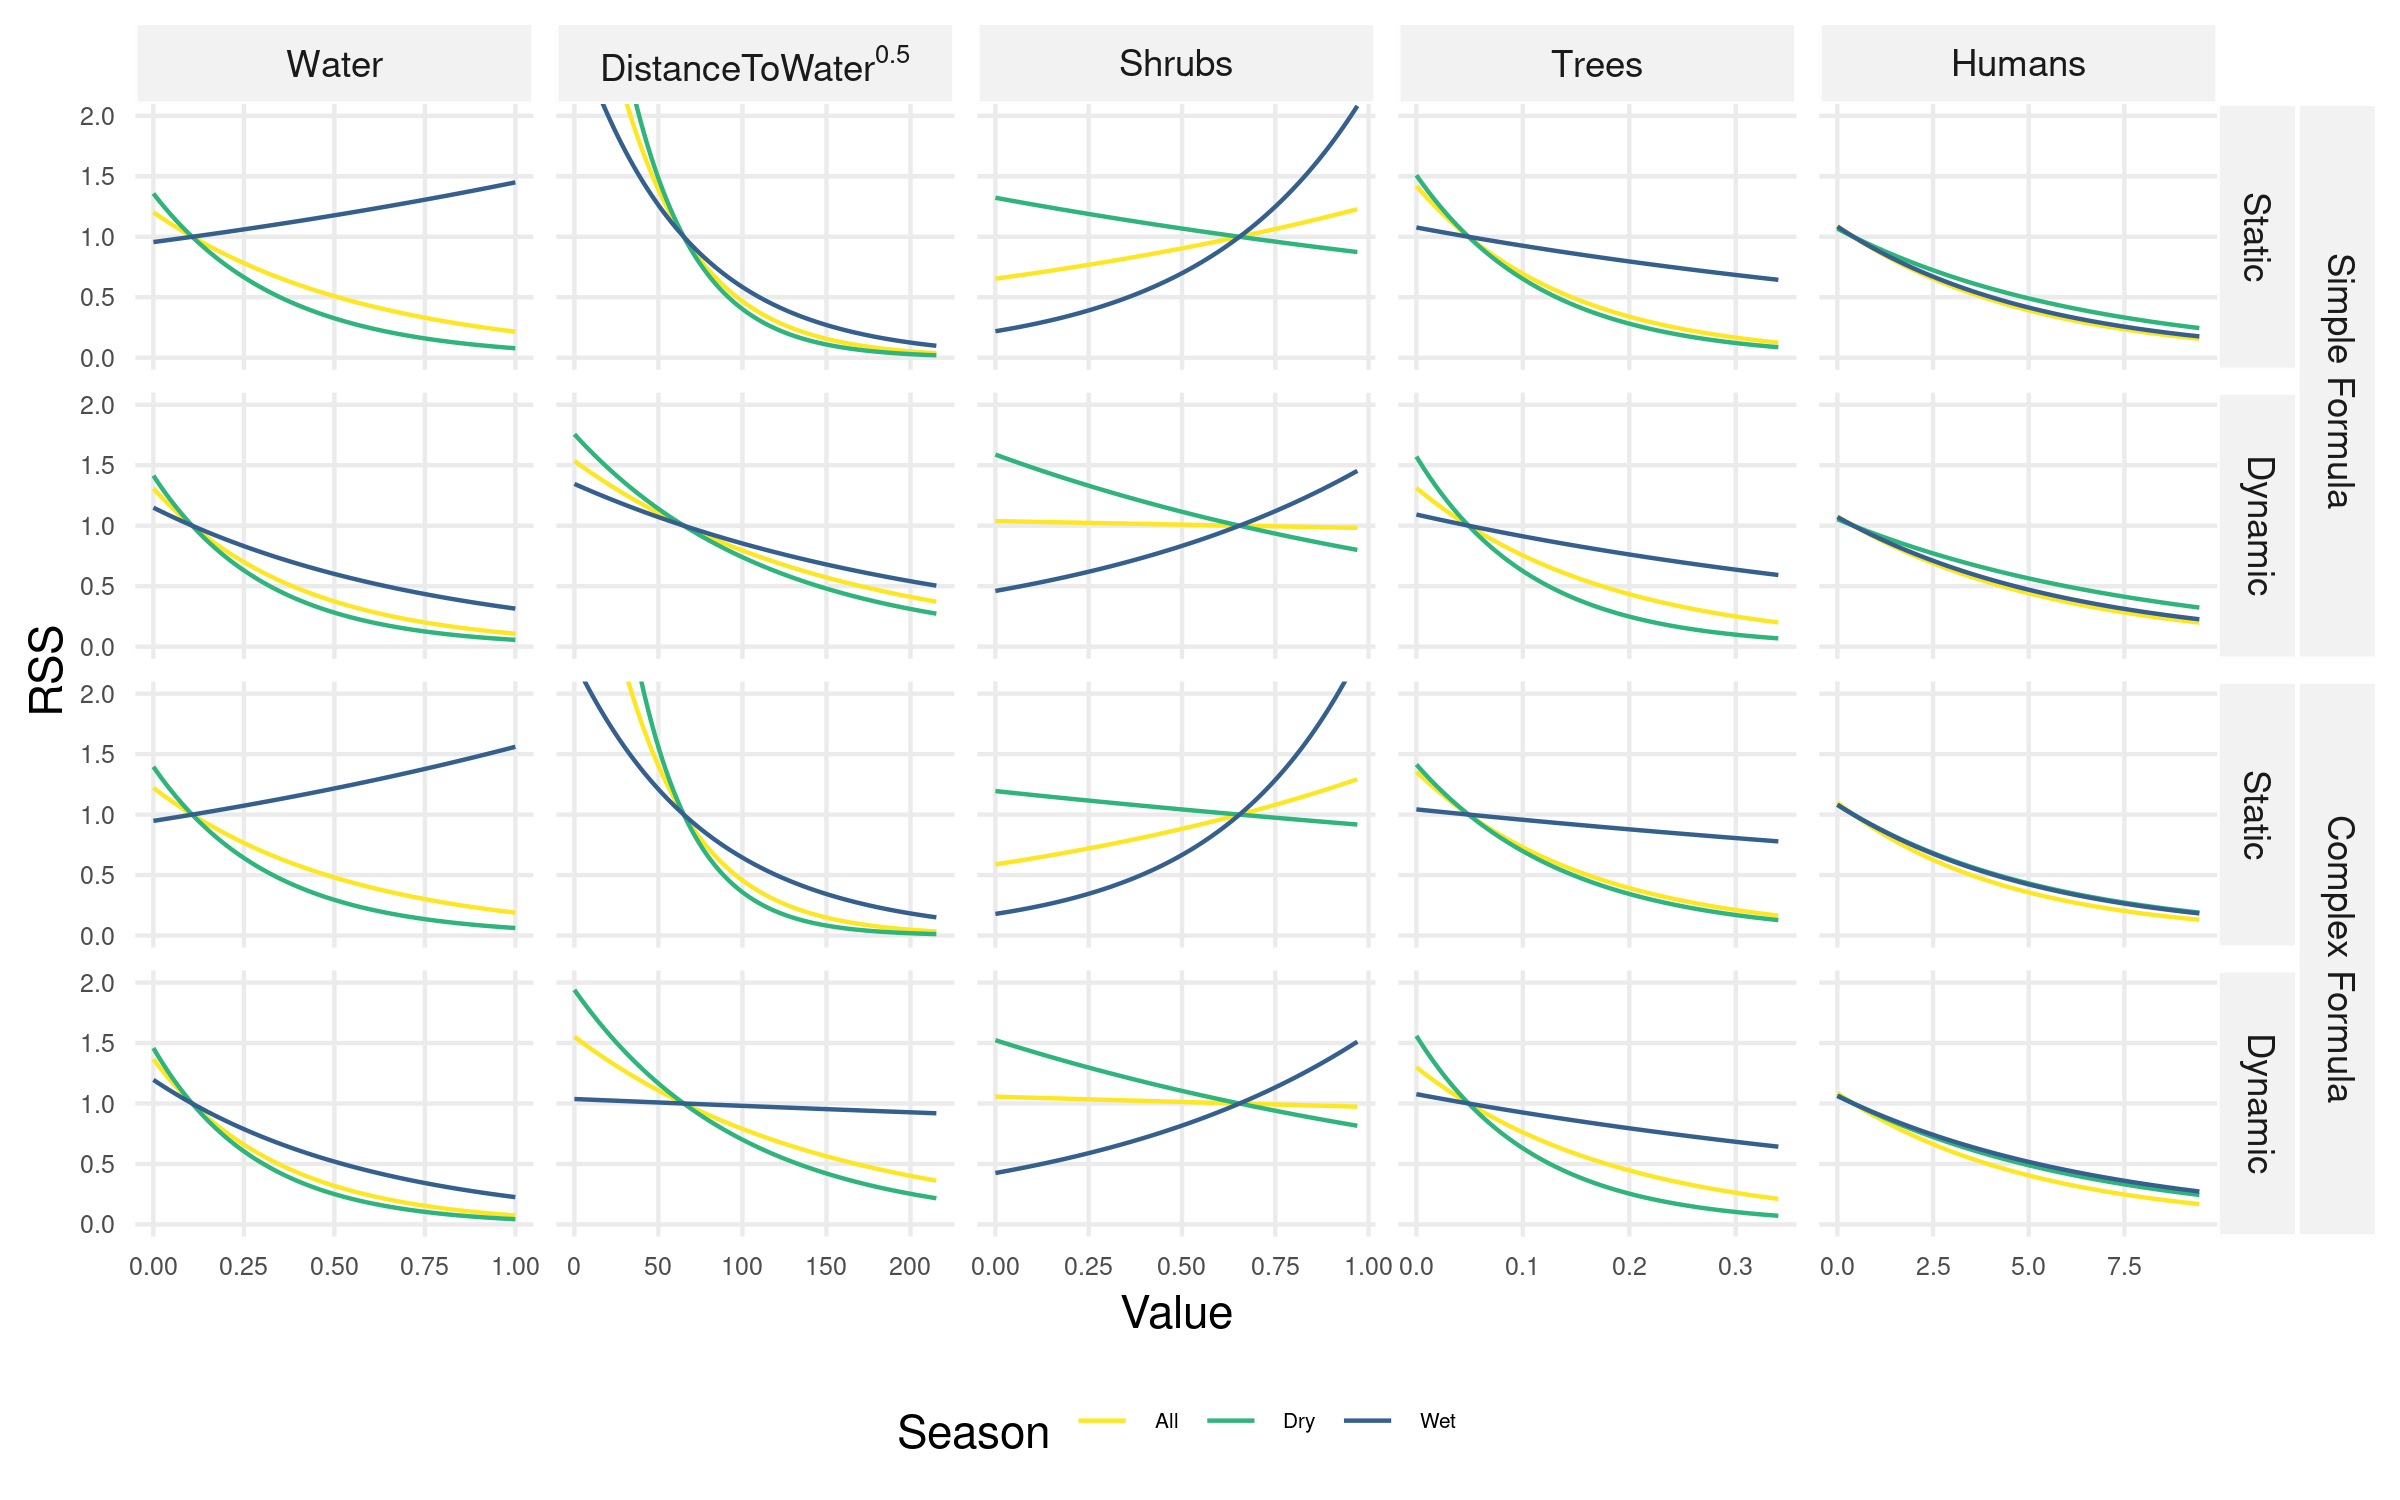
\includegraphics[width = \textwidth]{Figures/MovementModelInterpretation.png}
  \caption{Relative selection scores (RSS) with respect to environmental
  covariates. RSS scores were computed by comparing a location $x_1$ with
  average conditions to a location $x_2$ with average conditions but the
  respective covariate varied between its minimum and maximum observed value.
  Confidence intervals overlapped substantially, hence we omitted them from the
  figure to simplify the interpretation of the differences among
  configurations.}
  \label{MovementModelInterpretation}
 \end{center}
\end{figure}

%------------------------------------------------------------------------------
%	Appendix S7: Spearman Rank Correlation in Relation to Number of Random Steps
%------------------------------------------------------------------------------
\newpage
\section{Spearman's Rank Correlation in Relation to the Number of Random Steps}

\begin{figure}[htpb]
 \begin{center}
  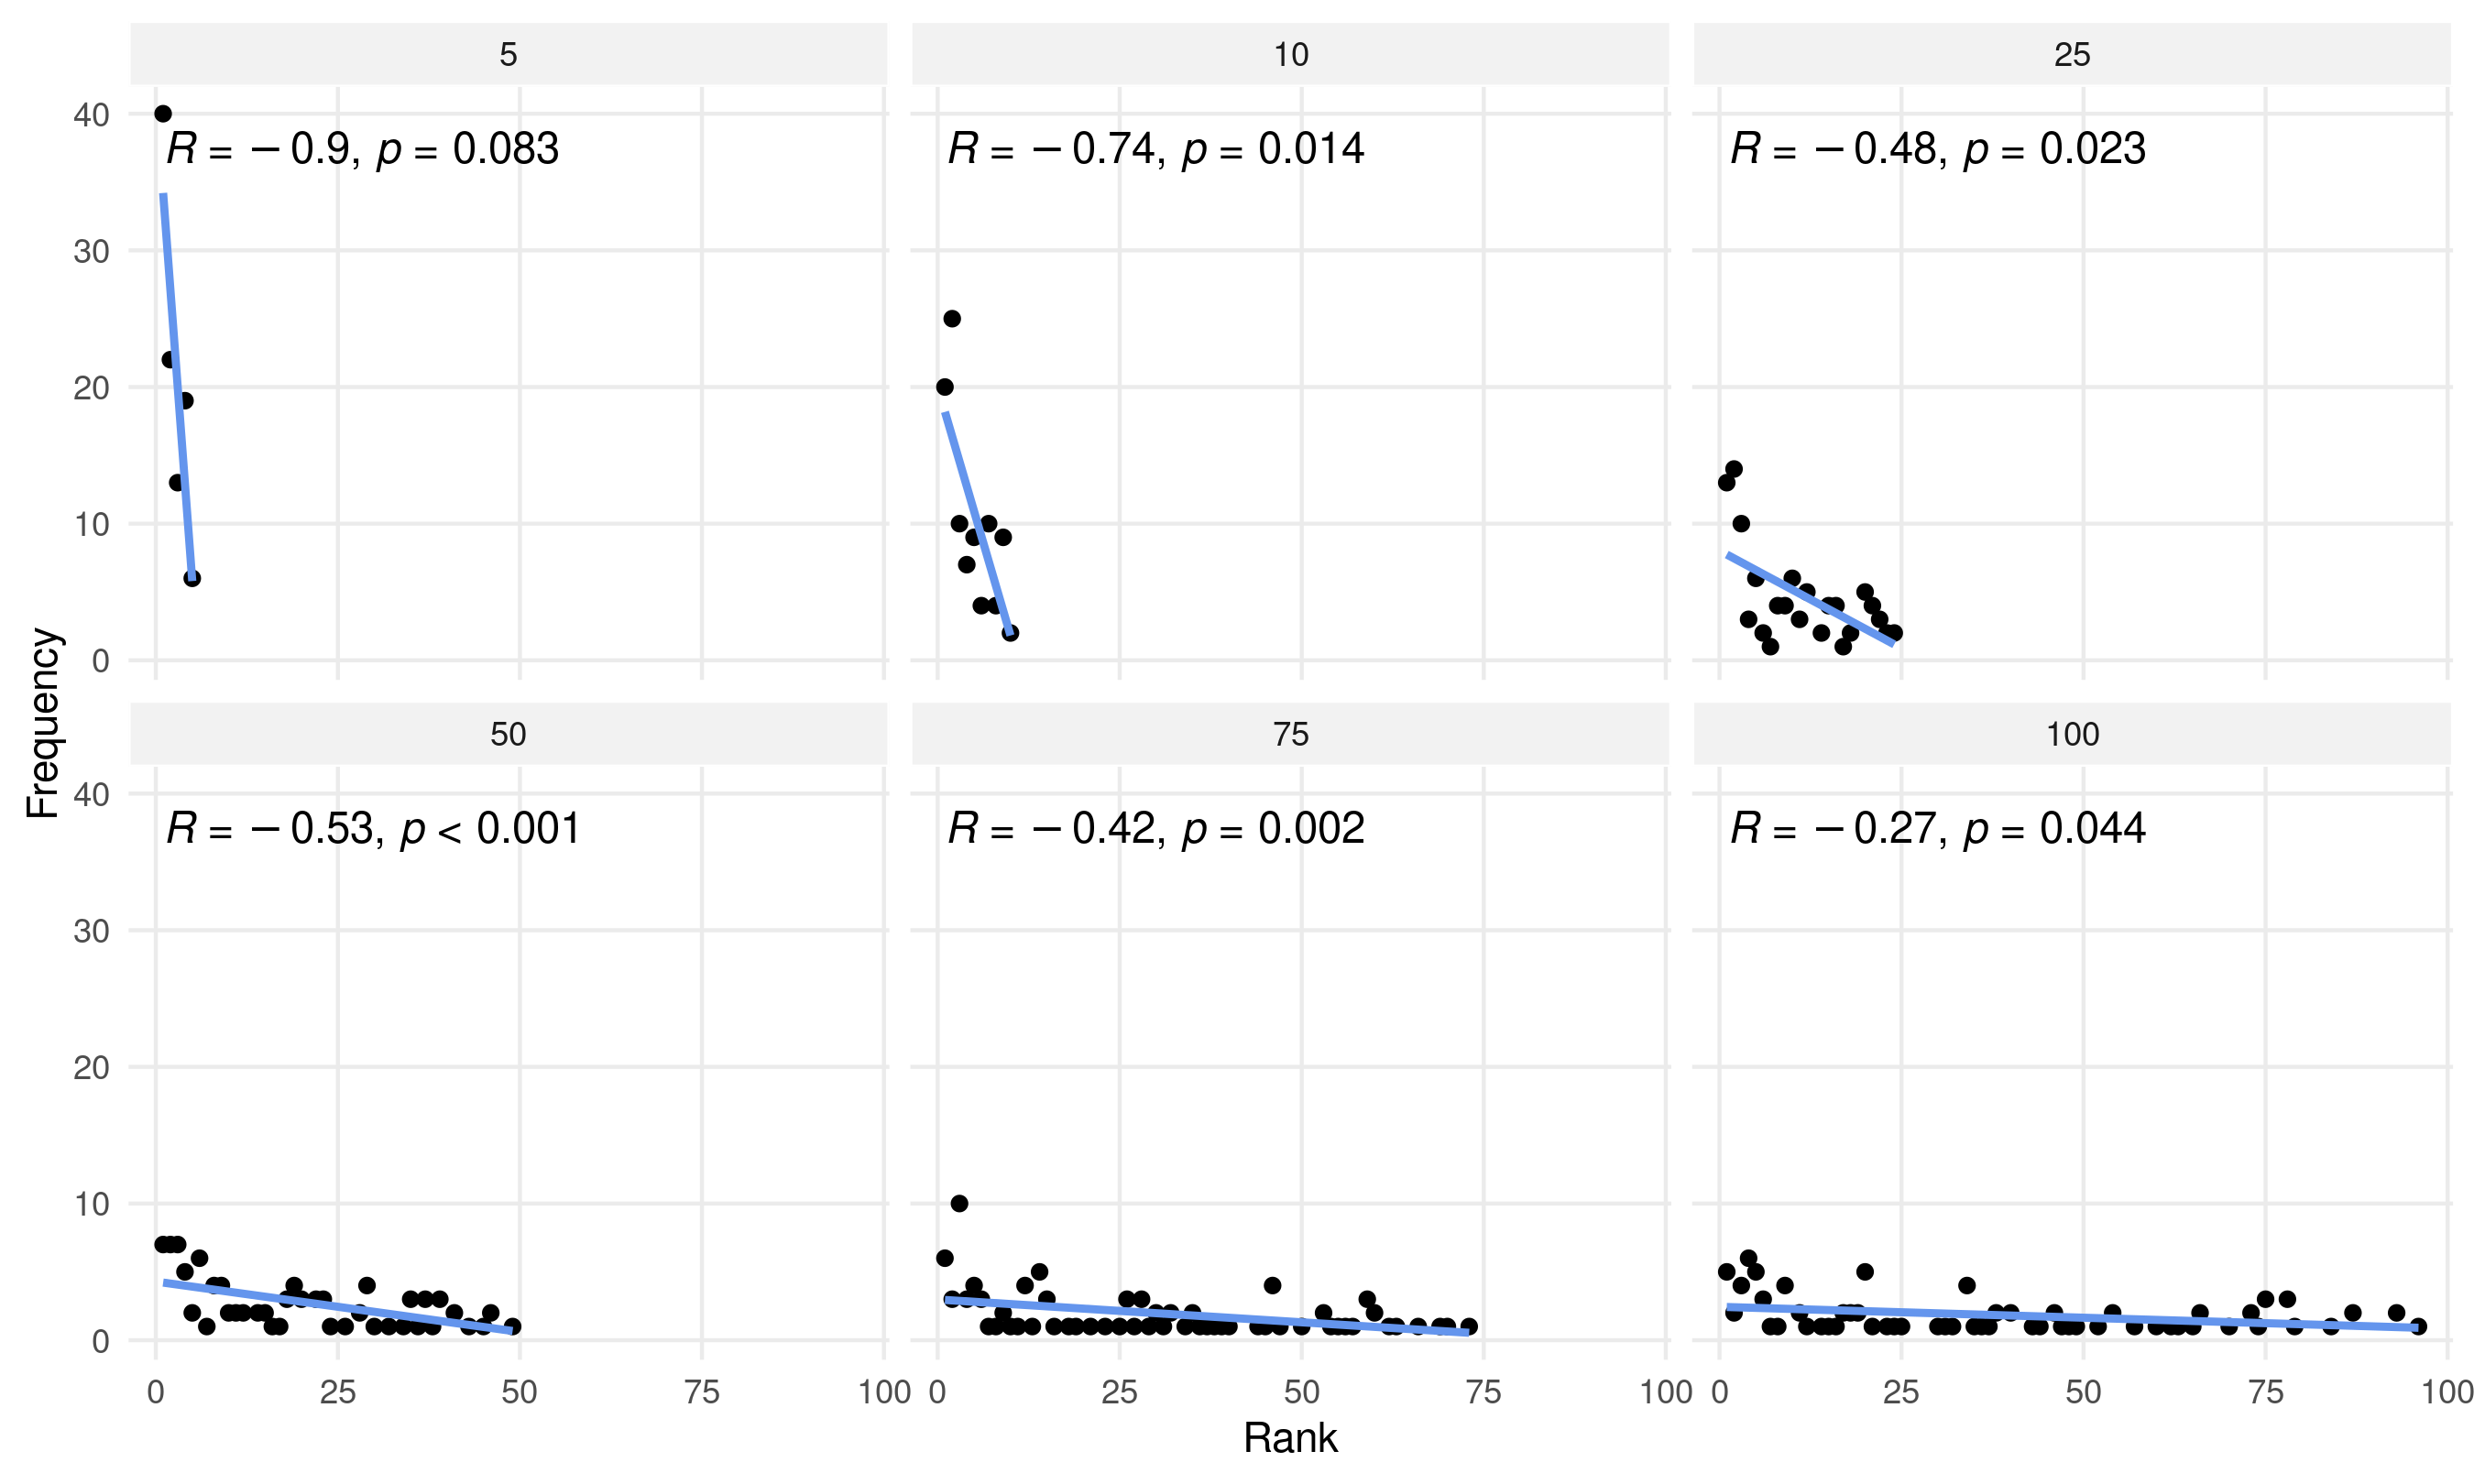
\includegraphics[width = \textwidth]{Figures/RankCorrelationNumberSteps.png}
  \caption{Illustration how the Spearman's rank correlation changes when the
  number of random steps per stratum is varied from 5 to 100 (facettes). The
  y-axis shows the frequency at which the observed step was assigned the rank
  indicated on the x-axis. A low rank indicates that the observed step was
  assigned a high probability of being chosen. The better the prediction, the
  more frequently the observed step should be assigned a low rank, thus
  resulting in negative Spearman's rank-correlation. However, it is obvious that
  the metric heavily depends on the number of random steps per stratum. If there
  are only a few random steps, the correlation is more likely to be negative.
  The show patterns are based on simulated data.}
  \label{RankCorrelationNumberSteps}
 \end{center}
\end{figure}

\ifSubfilesClassLoaded{%
  \newpage
  \begin{singlespacing}
  \ifthenelse{\boolean{usebiblatex}}{
    \begin{refcontext}[sorting=nyt]
    \printbibliography
    \end{refcontext}
  } {
    \bibliography{../LiteratureBibtex}%
  }
\end{singlespacing}
}{}

\end{document}
